% Options for packages loaded elsewhere
\PassOptionsToPackage{unicode}{hyperref}
\PassOptionsToPackage{hyphens}{url}
\PassOptionsToPackage{dvipsnames,svgnames,x11names}{xcolor}
%
\documentclass[
  10pt,
  dvipsnames,enabledeprecatedfontcommands]{scrartcl}
\usepackage{amsmath,amssymb}
\usepackage{lmodern}
\usepackage{iftex}
\ifPDFTeX
  \usepackage[T1]{fontenc}
  \usepackage[utf8]{inputenc}
  \usepackage{textcomp} % provide euro and other symbols
\else % if luatex or xetex
  \usepackage{unicode-math}
  \defaultfontfeatures{Scale=MatchLowercase}
  \defaultfontfeatures[\rmfamily]{Ligatures=TeX,Scale=1}
\fi
% Use upquote if available, for straight quotes in verbatim environments
\IfFileExists{upquote.sty}{\usepackage{upquote}}{}
\IfFileExists{microtype.sty}{% use microtype if available
  \usepackage[]{microtype}
  \UseMicrotypeSet[protrusion]{basicmath} % disable protrusion for tt fonts
}{}
\usepackage{xcolor}
\usepackage{graphicx}
\makeatletter
\def\maxwidth{\ifdim\Gin@nat@width>\linewidth\linewidth\else\Gin@nat@width\fi}
\def\maxheight{\ifdim\Gin@nat@height>\textheight\textheight\else\Gin@nat@height\fi}
\makeatother
% Scale images if necessary, so that they will not overflow the page
% margins by default, and it is still possible to overwrite the defaults
% using explicit options in \includegraphics[width, height, ...]{}
\setkeys{Gin}{width=\maxwidth,height=\maxheight,keepaspectratio}
% Set default figure placement to htbp
\makeatletter
\def\fps@figure{htbp}
\makeatother
\setlength{\emergencystretch}{3em} % prevent overfull lines
\providecommand{\tightlist}{%
  \setlength{\itemsep}{0pt}\setlength{\parskip}{0pt}}
\setcounter{secnumdepth}{5}
\newlength{\cslhangindent}
\setlength{\cslhangindent}{1.5em}
\newlength{\csllabelwidth}
\setlength{\csllabelwidth}{3em}
\newlength{\cslentryspacingunit} % times entry-spacing
\setlength{\cslentryspacingunit}{\parskip}
\newenvironment{CSLReferences}[2] % #1 hanging-ident, #2 entry spacing
 {% don't indent paragraphs
  \setlength{\parindent}{0pt}
  % turn on hanging indent if param 1 is 1
  \ifodd #1
  \let\oldpar\par
  \def\par{\hangindent=\cslhangindent\oldpar}
  \fi
  % set entry spacing
  \setlength{\parskip}{#2\cslentryspacingunit}
 }%
 {}
\usepackage{calc}
\newcommand{\CSLBlock}[1]{#1\hfill\break}
\newcommand{\CSLLeftMargin}[1]{\parbox[t]{\csllabelwidth}{#1}}
\newcommand{\CSLRightInline}[1]{\parbox[t]{\linewidth - \csllabelwidth}{#1}\break}
\newcommand{\CSLIndent}[1]{\hspace{\cslhangindent}#1}
%\documentclass{article}

% %packages
 \usepackage{booktabs}
\usepackage{subcaption}
\usepackage{multirow}
\usepackage{colortbl}
\usepackage{graphicx}
\usepackage{longtable}
\usepackage{ragged2e}
\usepackage{etex}
%\usepackage{yfonts}
\usepackage{marvosym}
%\usepackage[notextcomp]{kpfonts}
\usepackage[scaled=0.86]{helvet}
\usepackage{nicefrac}
\newcommand*{\QED}{\hfill \footnotesize {\sc Q.e.d.}}
\usepackage{floatrow}
%\usepackage[titletoc]{appendix}
%\renewcommand\thesubsection{\Alph{subsection}}

\usepackage[textsize=footnotesize]{todonotes}
\newcommand{\inbook}[1]{\todo[color=gray!40]{#1}}
\newcommand{\mar}[1]{\todo[color=blue!40]{#1}}
\newcommand{\raf}[1]{\todo[color=olive!40]{#1}}
%\linespread{1.5}
\newcommand{\indep}{\!\perp \!\!\! \perp\!}


\setlength{\parindent}{10pt}
\setlength{\parskip}{1pt}


%language
\usepackage{times}
\usepackage{t1enc}
%\usepackage[utf8x]{inputenc}
%\usepackage[polish]{babel}
%\usepackage{polski}

% modyfing quote environment

\usepackage[T1]{fontenc}             % Required for correct quotes with ""

\renewenvironment{quote}
{\list{}{\leftmargin=1em\rightmargin=1em}\item[]``}
{''\endlist}




%AMS
\usepackage{amsfonts}
\usepackage{amssymb}
\usepackage{amsthm}
\usepackage{amsmath}
\usepackage{mathtools}

\usepackage{geometry}
 \geometry{a4paper,left=35mm,top=20mm,}


%environments
\newtheorem{fact}{Fact}



%abbreviations
\newcommand{\ra}{\rangle}
\newcommand{\la}{\langle}
\newcommand{\n}{\neg}
\newcommand{\et}{\wedge}
\newcommand{\jt}{\rightarrow}
\newcommand{\ko}[1]{\forall  #1\,}
\newcommand{\ro}{\leftrightarrow}
\newcommand{\exi}[1]{\exists\, {_{#1}}}
\newcommand{\pr}[1]{\mathsf{P}(#1)}
\newcommand{\cost}{\mathsf{cost}}
\newcommand{\benefit}{\mathsf{benefit}}
\newcommand{\ut}{\mathsf{ut}}

\newcommand{\dkl}{D_{\mathsf{KL}}} % trying to add the definition of \dkl

\newcommand{\odds}{\mathsf{Odds}}
\newcommand{\ind}{\mathsf{Ind}}
\newcommand{\nf}[2]{\nicefrac{#1\,}{#2}}
\newcommand{\R}[1]{\texttt{#1}}
\newcommand{\prr}[1]{\mbox{$\mathtt{P}_{prior}(#1)$}}
\newcommand{\prp}[1]{\mbox{$\mathtt{P}_{posterior}(#1)$}}

\newcommand{\s}[1]{\mbox{$\mathsf{#1}$}}


\newtheorem{q}{\color{blue}Question}
\newtheorem{lemma}{Lemma}
\newtheorem{theorem}{Theorem}
\newtheorem{definition}{Definition}        % trying to add the def. environment




%technical intermezzo
%---------------------

\newcommand{\intermezzoa}{
	\begin{minipage}[c]{13cm}
	\begin{center}\rule{10cm}{0.4pt}



	\tiny{\sc Optional Content Starts}
	
	\vspace{-1mm}
	
	\rule{10cm}{0.4pt}\end{center}
	\end{minipage}\nopagebreak 
	}


\newcommand{\intermezzob}{\nopagebreak 
	\begin{minipage}[c]{13cm}
	\begin{center}\rule{10cm}{0.4pt}

	\tiny{\sc Optional Content Ends}
	
	\vspace{-1mm}
	
	\rule{10cm}{0.4pt}\end{center}
	\end{minipage}
	}
%--------------------






















\newtheorem*{reply*}{Reply}
\usepackage{enumitem}
\newcommand{\question}[1]{\begin{enumerate}[resume,leftmargin=0cm,labelsep=0cm,align=left]
\item #1
\end{enumerate}}

\usepackage{float}

% \setbeamertemplate{blocks}[rounded][shadow=true]
% \setbeamertemplate{itemize items}[ball]
% \AtBeginPart{}
% \AtBeginSection{}
% \AtBeginSubsection{}
% \AtBeginSubsubsection{}
% \setlength{\emergencystretch}{0em}
% \setlength{\parskip}{0pt}






\usepackage[authoryear]{natbib}

%\bibliographystyle{apalike}



\usepackage{tikz}
\usetikzlibrary{positioning,shapes,arrows}

\ifLuaTeX
  \usepackage{selnolig}  % disable illegal ligatures
\fi
\IfFileExists{bookmark.sty}{\usepackage{bookmark}}{\usepackage{hyperref}}
\IfFileExists{xurl.sty}{\usepackage{xurl}}{} % add URL line breaks if available
\urlstyle{same} % disable monospaced font for URLs
\hypersetup{
  pdftitle={Many roads to higher-order probability},
  colorlinks=true,
  linkcolor={Maroon},
  filecolor={Maroon},
  citecolor={Blue},
  urlcolor={blue},
  pdfcreator={LaTeX via pandoc}}

\title{Many roads to higher-order probability}
\author{}
\date{\vspace{-2.5em}}

\begin{document}
\maketitle

\textbf{DISCLAIMER:} An .Rmd file containing all \textbf{\textsf{R}}
code for the computations used in the paper has also been submitted for
the perusal of the referees.

\begin{quote}
\textbf{Wordcount: 20k}
\end{quote}

\begin{quote}
\textbf{Abstract.} Precise probabilism (PP) has it that   a rational agent's (RA)  uncertainty is to be represented as a single probability measure. The view has been criticized on the ground that RA's degrees of belief are not appropriately evidence-responsive, especially when evidence is scant. Accordingly, an alternative view---imprecise probabilism (IP)---has been proposed, on which RA's uncertainty is to be represented by a set of probability measures, rather than a unique one. This view runs into problems as well. The positive proposal in which this paper goes beyond this debate, roughly, is this: instead of using IP and running into its own difficulties, why not use methods that Bayesian statistics is already familiar with? Let's think about the uncertainty about a proposition in terms of parameter uncertainty, where this parameter is the right probability that one should assign to that proposition (be it chance, the sole rational probability given the evidence, or what have you, let's leave the philosophical discussion open). Once we do this, there are tools that we can use to explain how the framework can handle both the motivations for departing from PP and the difficulties that IP runs into. This higher-order approach allows for an appropriate degree of evidence-responsiveness, correctly resolves known tricky comparative probability cases, does not run into belief inertia, allows for information-theoretic explications of weight and a (strictly proper) inaccuracy measure, and opens a path to opinion pooling methods that go beyond and lead to higher accuracy than the usual proposals on the market. 

\end{quote}

\hypertarget{introduction}{%
\section{Introduction}\label{introduction}}

Precise probabilism (PP) has it that a rational agent's (RA) uncertainty
is to be represented as a single probability measure. The view has been
criticized on the ground that RA's degrees of belief are not
appropriately evidence-responsive, especially when evidence is scant.
Accordingly, an alternative view---imprecise probabilism (IP)---has been
proposed, on which RA's uncertainty is to be represented by a set of
probability measures, rather than a unique one.

Unfortunately, this view runs into problems as well. It still does not
seem to be sufficiently evidence-responsive, it is claimed to get
certain comparative probability judgments wrong, it seems to be unable
to model learning with the starting point is complete lack of
information, it is not rich enough to model the notion of weight of
evidence, and notoriously there exist on inaccuracy measure of an
imprecise credal stance if the measure is to satisfy certain
straightforward formal conditions. Moreover, while it seems to handle
some cases of opinion pooling better than PP, it still can't capture the
phenomenon of synergy, where slightly disagreeing sources or experts
jointly in some sense seem to improve the epistemic situation.

The main claim of this paper is that the way forward is to use
higher-order probabilities. The key idea is that uncertainty is not a
single-dimensional thing to be mapped on a single one-dimensional scale
like a real line and that it's the whole shape of the whole distribution
over parameter values that should be taken under consideration. This
guiding idea can be used to resolve many problems and philosophical
puzzles raised in the debate between PP and IP.

While in principle the paper could have been made shorter or smoother by
focusing on just some of the problems, I think the best way to show the
force of this approach is to emphasize the unity with which it handles
many different dimensions of the debate, so the reader should prepare
herself for multiple arguments flying back and forth in an initially
seemingly disconnected manner. I ask the reader for some patience: in
the end, it will be clear that, in the words of Dirk Gently, it's all
connected.

Given the convoluted structure of the paper, some heads up are needed
(we will also make short stops here and there to look at the map and ask
where we are and where we are going). Section \ref{sec:imprecision}
describes the foundation of the disagreement: precise probabilism, the
challenge of evidence responsiveness, and how imprecise probabilism is
supposed to improve on the situation. Section \ref{sec:epistemic}
focuses on problems that imprecise probabilism (and sometimes precise
probabilism too) runs into. Admittedly, this is quite a lot of set-up,
but to fully appreciate how my approach handles the difficulties, we
first need to give those problems the attention that they deserve. In
Section \ref{sec:rethinking} we do some soul-searching, looking at how
basic elements of the positive proposal that will follow can be found in
the literature, often in the writings of the proponents or critics of
imprecise probabilism themselves. Finally, in Section \ref{sec:positive}
I introduce the positive proposal and explain how it can be used to
overcome all the problems discussed up to that point. As in the process
I propose an information-theoretic inaccuracy measure, I also prove its
strict propriety in the appendix.

\hypertarget{imprecision-and-evidence-responsiveness}{%
\section{\texorpdfstring{Imprecision and evidence responsiveness
\label{sec:imprecision}}{Imprecision and evidence responsiveness }}\label{imprecision-and-evidence-responsiveness}}

According to classical Bayesian epistemology,
\textbf{precise probabilism} (PP), a rational agent's (RA) degrees of
belief are to be represented by means of a single probability measure
and RA is supposed to have a credence in every proposition she
entertains. As a simple example, consider coin tossing and RA's credal
state with respect to (H):

\begin{center}
\begin{tabular}{lp{9cm}}
(H) & The outcome of the next toss will be heads,
\end{tabular}
\end{center}

\noindent in the following scenario:

\begin{center}
\begin{tabular}{lp{9cm}}
(Fair coin) & RA is about to toss a fair coin.
\end{tabular}
\end{center}

\noindent The sample space of interest here is \(S = \{ H, \neg H\}\),
and RA's credal position, intuitively, can be represented as a single
probability measure \(\mathsf{P}\) with
\(\mathsf{P}(H) = \mathsf{P}(\neg H)=.5\). But now, suppose the
situation is somewhat different:

\begin{center}
\begin{tabular}{lp{9cm}}
(Unknown bias) & RA is about to toss a coin whose bias is unknown.
\end{tabular}
\end{center}

Here, the preciser---if pressed to come up with a single probability
measure---might say that following the principle of insufficient
evidence they assign equal probability (density) to each possible bias,
and the expected value calculations lead them again to \(\pr{H}=.5\).

Here is an assumption that might seem initially plausible:

\begin{tabular}{lp{11cm}}
(Locality) & RA's credal stance (in a wide, non-technical sense) about a proposition is to be captured by whatever probability (or probabilities) she assigns to it, and does not depend on what probabilities RA assigns to logically independent  propositions.
\end{tabular}

\noindent The idea here is that if one proposes a formal model of RA's
credal stance towards a proposition, it should be functional---whatever
object \(o\) the model assigns to \(H\), \(o\) should capture RA's
attitude towards \(H\). On PP, the model is a unique probability measure
and the object assigned to \(H\) is the probability of \(H\).

For now, let's see how far we can get with (Locality). In the present
context it entails that as far as RA's stance towards \(H\) is
concerned, restricting attention to propositions built over \(S\) is
fine. But if we do so, the preciser does not distinguish between (Fair
coin) and (Unknown bias). This inability to capture an important
epistemological difference, the impreciser insists, is a serious
limitation. Intuitively, a precise stance is not justified by the very
scant evidence available.\footnote{Here's another argument for RA's
  indifference about \(H\) and RA's having a precise credence in \(H\)
  set to .5 being intuitively different states. Indifference is not
  sensitive to sweetening, that is, improving the chances of \(H\) only
  slightly. If RA doesn't know what the bias of the coin is, learning
  that it now has been slightly modified to increase the chance of \(H\)
  by .001, might still leave RA unwilling to bet in a bet on \(H\) that
  would've been fair even if the actual chance of \(H\) was .5 and not
  .001. The same sweetening, however, would make RA bet on \(H\) if
  their original credal stance towards \(H\) was the precise credence
  equal .5.}

\textbf{Imprecise probabilism} (IP), in the now classical version of the
view, holds that RA's credal stance towards \(H\) is to be represented
by means of a set of probability measures (\emph{representor})
\(\mathbb{P}\), rather than a single measure \(\mathsf{P}\). The
underlying intuition is that given the evidence, the representor should
include all and only those probability measures which are
\textbf{compatible with this evidence.} While the impreciser in (Fair
coin) would take RA's credal state towards \(N\) to be captured by
\(\{\mathsf{P}\}\), where \(\mathsf{P}\) is as in the preciser's
approach, in (Unknown bias) they would rather represent RA's credal
state by means of the set of all probabilistic measures defined on
\(S\), as none of them is excluded by the available
evidence.\footnote{Crucially, on this position it is not the case that the set represents admissible options and RA can legitimately pick any precise measure from the set. Rather, RA's credal stance is essentially imprecise and has to be represented by means of the whole set.}
Their formal representation, therefore, seems to preserve the intuitive
difference in the probabilities that the evidence seems to exclude in
(Fair coin) and in (Unknown bias).\footnote{Some sources related to the
  development of imprecise probabilism are (B. C. V. Fraassen, 2006;
  Gärdenfors \& Sahlin, 1982; James M. Joyce, 2005; J. Kaplan, 1968;
  Keynes, 1921; Levi, 1974; Sturgeon, 2008; Walley, 1991), (Bradley,
  2019) is a good source of literature.} In this sense, the RA's credal
state as modeled by IP seems to be more
\textbf{responsive to evidence (or lack thereof)} than when modeled from
the perspective of PP.

Here's another reason why you might consider IP. If you think that
\textbf{completeness is too strong for comparative probability}, this is
a reason to go beyond PP. Since completeness holds for the comparison of
real numbers, if you accept that RA's credal stance towards the
propositions they consider is to be represented by real numbers, one for
each proposition, it follows that any two propositions can be
unambiguously compared. If you think evidence sometimes might be weak
enough not to sanction any preference, or that RA's is sometimes allowed
to suspend judgment about \(X\), and this suspension is different from
simply taking \(\mathsf{P}(X)=.5\), you have a reason to depart from PP.
This is in line with the distinction between indifference and indecision
(J. Kaplan, 1968): RA is indifferent between \(A\) and \(B\) if they
somehow determined them to be equally likely, while if RA can't make up
their mind without such determination, RA is undecided about \(A\) and
\(B\). This distinction seems impossible to preserve while sticking to
PP (Bradley, 2019). In contrast, a representor can---in a
supervaluationist manner---capture both
\textbf{determinate and indeterminate stances} towards various
propositions. For instance, if every probabilistic measure in the
representor assigns a higher value to \(H_1\) rather than \(H_2\), we
can take the RA to definitely hold that \(H_1\) is more probable than
\(H_2\).

Yet another problem for PP arises when we consider
\textbf{combining or aggregating probabilistic opinions} of members of
groups, as formulating a sensible method thereof for PP turned out to be
challenging. For instance, a seemingly intuitive constraint is that if
every member agrees that \(X\) and \(Y\) are probabilistically
independent, the aggregated credence should respect this. But this is
hard to achieve if we stick to PP (Dietrich \& List, 2016). For
instance, linear pooling does not respect this. Consider probabilistic
measures \(p\) and \(q\) such that \(p(X) = p(Y) = p(X\vert Y) = 1/3\)
and \(q(X) = q(Y) = q(X\vert Y) = 2/3\). On both measures, taken
separately, \(X\) and \(Y\) are independent. Now take the average,
\(r=p/2+q/2\). Then \(r(X\cap Y) = 5/18 \neq r(X)r(Y)=1/4\).
Independence is not preserved.

A nice related example comes from (Gallow, 2018). Al and Bert are two
local weather forecasters. At least when it comes to the question of
whether it will rain, they are both quite reliable. And their forecasts
tend, for the most part, to agree. When they disagree, it is sometimes
Al and sometimes Bert that gets closer to the truth. One reason they
agree so often is that they discuss their provisional forecasts with one
another before deciding upon a final forecast. Today RA is wondering
whether it will rain; and RA has not yet checked the forecasts. Should
RA be certain that Al and Bert will issue identical forecasts? Al and
Bert have in the past disagreed with each other, so RA should not be
absolutely certain that they will issue identical forecasts today, RA's
credence (if we are to represent her stance within PP) should satisfy:
\begin{align} \label{eq:gal1}
\pr{A=B} & <1
\end{align} \noindent Given that Al forecasts that the chance of rain is
\(a\) and RA doesn't know anything about Bert, how confident should RA
be that it will rain? A plausible answer is ``\(a\)''---this not only
sounds plausible, but is endorsed for various epistemic experts by many
(Elga, 2007; B. C. van Fraassen, 1984; Gaifmam, 1988; Lewis, 1980).
\begin{align} \label{eq:gal2}
\pr{r\vert A=a}  = a  &  \,\,\,\, \pr{r\vert B=b}  = b
\end{align} If Al and Bert disagree, though, the plausible answer, is
that RA's confidence in rain should be some weighted average of \(a\)
and \(b\) (with weights determined by Al and Bert's prior reliability,
perhaps). \begin{align} \label{eq:gal3}
\forall a,b \, \pr{r \vert A =a, B = b} & =  \alpha a + \beta b
\end{align} \noindent However, if \(r\) is an arbitrary proposition and
\(A\) and \(B\) are random variables taking values in the unit interval,
there is no probability measure \(\mathsf{P}\) such that
\eqref{eq:gal1}, \eqref{eq:gal2}, and \eqref{eq:gal3} all hold.

There have been some attempts to improve on the situation (List \&
Pettit, 2011), but opinion pooling still remains a challenge for PP. The
problems with aggregation are used by Stewart \& Quintana (2018) as an
argument for imprecise probabilities, as IP offers a potential way out.
Instead of combining probability measures into one aggregate opinion,
consider the set containing them all as the aggregation result. Also,
there does not seem to be any middle ground between using precise
probabilities and using the representor if we wish to preserve the
expressive power the need for which motivated IP to start with. For
instance, there are less complex representations of evidence
responsiveness, but they fail to adequately
\textbf{capture dependencies between propositions, such as logical dependencies}.
To consider one candidate, let \(\mathbb{P}(X)\) be the set of all
probabilities assigned to proposition \(X\) by the measures in
\(\mathbb{P}\), call \(inf(\mathbb{P}(X))\) (\(sup (\mathbb{P}(X))\))
the lower (upper) envelope. Note that representing RA's credal state
with respect to \(H\) by \(\mathbb{P}(X)\) or by the pair
\((inf(\mathbb{P}(X)),sup (\mathbb{P}(X))\) does not do justice to the
dependencies between propositions. Even in a fairly simple case of
(Uknown bias), such representations fail to capture the fact that for
any \(\mathsf{P}\in \mathbb{P}, \mathsf{P}(\neg H) = 1- \mathsf{P}(H)\),
that is, that according to the agent \(H\) and its negation exclude each
other.

Before we move on, two moves typically made by the proponents of IP that
will be used later on are worth mentioning. First, \textbf{learning} in
IP is a natural extension of the classical Bayesian approach. When faced
with new evidence \(E\) between time \(t_0\) and \(t_1\), RA's
representor should be updated point-wise: simply run the standard
Bayesian updating on each probability measure in the representor:
\begin{align*} \label{eq:updateRepresentor}
\mathbb{P}_{t_1} = \{\mathsf{P}_{t_1}\vert \exists\, {\mathsf{P}_{t_0} \!\in  \mathbb{P}_{t_0}}\,\, \forall\, {H}\,\, \left[\mathsf{P}_{t_1}(H)=\mathsf{P}_{t_0}(H \vert E)\right] \}.
\end{align*}

Second, at various points we will be using priors, and the ability to
express agnosticism or complete lack of information will play an
important role. Unless we plan to go subjectivist, the main stream of
Bayesianism recommend the \textbf{maximum entropy rule} (MaxEnt) for the
choice of the prior distribution, which requires one to start with a
distribution that---given the evidence available---is maximally
noncommittal with regard to missing information (Jaynes, 2003;
Williamson, 2010). While often we will deploy such priors for
illustrative purposes, this choice is extraneous to the representation
methods described in this paper.\footnote{This choice of priors has
  been, for instance, challenged (Konek, 2013) on the grounds that while
  MaxEnt might indeed select the most appropriate distribution given the
  (lack of) evidence, if the goal of the priors is not to represent the
  lack of evidence, but to optimize the expected accuracy, a different
  prior selection rule, MaxSen, which recommends choosing the prior that
  minimizes the variance in expected accuracy, should be used. Given
  that it requires extensive optimization and its lack of impact on the
  literature, it is not in wide use among Bayesian statisticians.
  Another, more common approach, for cases in which evidential
  constraints are very weak involves regularizing priors, which have the
  advantage of being less malleable by the data than uniform priors, and
  so are less susceptible to over-fitting.}

We now have seen the key problems posed to PP, and how IP is supposed to
avoid them. Unfortunately, IP faces other objections. Some of them have
to do with decision theory, but in this paper we focus on those more
directly connected with epistemology and epistemic values.

\hypertarget{epistemic-challenges-to-imprecise-probabilism}{%
\section{\texorpdfstring{Epistemic challenges to imprecise probabilism
\label{sec:epistemic}}{Epistemic challenges to imprecise probabilism }}\label{epistemic-challenges-to-imprecise-probabilism}}

\hypertarget{more-evidence-responsiveness}{%
\subsection{More evidence
responsiveness}\label{more-evidence-responsiveness}}

If, as IP suggests, RA's credal stance towards \(H\) is to be
represented as a set of measures over \(S\), it seems that still it is
not too hard to come up with cases in which RA's evidential situation is
different, but between which IP fails to distinguish. Consider the
following scenario:

\begin{center}
\begin{tabular}{lp{9cm}}
(Two biases) & RA is about to toss a coin whose bias is either .4 or .6.
\end{tabular}
\end{center}

\noindent Perhaps you are inclined to say that in (Two biases) RA's
credal stance should be represented by \(\mathsf{P}_1, \mathsf{P}_2\)
such that \(\mathsf{P}_1(H)=.4\) and \(\mathsf{P}_2(H)=.6\). But now,
how---on IP---do you represent the following situation?

\begin{center}
\begin{tabular}{lp{9cm}}
(Two unbalanced biases) & RA is about to toss a coin whose bias is either .4 or .6, and bias .4 is three times  more likely than .6.
\end{tabular}
\end{center}

\noindent As long as you want to talk about measures defined over \(S\)
only, you will have hard time representing this
difference.\footnote{Perhaps, you can also start talking about higher-order probabilities over the members of  a representor, by saying that RA's stance towards $H$ is---at least in (Two unbalanced biases)---is  now to be represented by the representor $\{\mathsf{P}_1, \mathsf{P}_2\}$ as before, but joint with the probability over these expressing the true chances, $\mathsf{P}$, such that $\mathsf{P}(\mathsf{true\,\, chance \,\, of \,\, heads } = \mathsf{P}_1) =\nicefrac{3}{4}$ and $\mathsf{P}(\mathsf{true\,\, chance \,\, of \,\, heads } = \mathsf{P}_2) =\nicefrac{1}{4}$. Note this means that on this approach, to distinguish between  fairly straightforwardly different epistemic situations, we already need to assign probabilities to probabilities, in that sense going higher-order. Alternatively, you might want to recourse to a single probability measure $\mathsf{P}$ over chance hypotheses $ch(H)=x$ such that $\mathsf{P}(ch(H)=.4)=\nicefrac{3}{4}$, $\mathsf{P}(ch(H)=.6)=\nicefrac{1}{4}$ and $\mathsf{P}(ch(H)=x)=0$ for $x \not \in \{.4, .6\}$. Either way, you're conceding that RA's stance towards $H$ is to be represented by a probabilistic measure towards propositions other than those built over $S$.}

\hypertarget{comparisons-revisited}{%
\subsection{Comparisons revisited}\label{comparisons-revisited}}

Here is how Rinard (2013) uses the supervaluationist comparison method
to argue against IP. Suppose RA knows of two urns, \textsf{GREEN} and
\textsf{MYSTERY}. RA is certain \textsf{GREEN} contains only green
marbles, but has no information relevant to the colors of the marbles in
\textsf{MYSTERY}. A marble will be drawn at random from each. RA should
be certain that the marble drawn from \textsf{GREEN} will be green
(\(G\)), and RA should be more confident about this than about the
proposition that the marble from \textsf{MYSTERY} will be green (\(M\)).
If, however, in line with IP, for each \(r\in [0,1]\) RA's representor
contains a \(\mathsf{P}\) with \(\pr{M}=r\), then it also contains one
with \(\pr{M}=1\). This means that it is not the case that for any of
RA's representor \(\mathsf{P}\), \(\mathsf{P}(G) > \mathsf{P}(M)\), that
is, it is not the case that RA is more confident of \(G\) than of \(M\).
This, Rinard posits, is highly counter-intuitive, and so, if IP
subscribes to the supervaluationists truth conditions for comparative
probability judgments (as it seems to), it runs into trouble.

\hypertarget{belief-inertia}{%
\subsection{Belief inertia}\label{belief-inertia}}

Here is another objection (Levi, 1980), which seems to indicate that IP
has hard time modeling from the state of (near) ignorance in the
following sense. Suppose RA starts tossing the coin starting with
knowing only that the coin bias is in \([0,1]\) (Stage
0)\footnote{The argument also works with the open interval $(0,1)$ as well, and in fact has a bite as long as the representor includes a measure which assigns either 1 or 0 to $H$.}
and later on observes the outcome of ten tosses, half of which turn out
to be heads. This is evidence for the real bias being around .5 (Stage
1)---not very strong evidence, but evidence nonetheless.

First, note that PP, if the principle of insufficient evidence is
deployed, starts with \(\mathsf{P}_0(H)=.5\) in Stage 0 and ends with
\(\mathsf{P}_1(H)=.5\) in Stage 1---whatever the epistemological
difference with respect to \(H\) there is between these two stages, it's
not captured by RA's precise credence over \(S\).

Second, however, note that the case is also problematic for IP if RA's
credal state in Stage 0 is to be modeled by the set of all possible
probability measures over \(S\). Of course, once RA moves to Stage 1,
each particular measure from the Stage 0 representor gets updated to a
different one that assigns a value closer to .5 to \(H\), but also each
measure in Stage 0 can be reached from another measure in Stage 0 by
updating on the evidence available in Stage 1. Thus, if RA's is to
update their representor point-wise, they end up with the same
representor set. Whatever they learned by observing five heads in ten
tosses, is not captured by the formal representation proposed by IP.

Here's another example of inertia posed by Rinard. Suppose RA's is faced
with an urn such that either all the marbles in the urn are green
(\(H_1\)), or exactly one tenth of the marbles are green (\(H_2\)). In
accordance with the wide interval view, RA has credence \([0,1]\) in
each. RA then learns that the marble drawn at random from the urn is
green (\(E\)) After conditionalizing each function in RA's representor
on \(E\), RA has exactly the same spread of values for \(H_1\) that they
did before learning \(E\), namely \([0,1]\), and in fact this does not
depend on how many marbles are sample from the urn and found to be
green.

Some replies on behalf of IP are available. One might admit that vacuous
priors are trivial and should not be used, while claiming that the
framework gives the right results when the priors are non-vacuous.
Another strategy is to say that in a state of complete ignorance a
special updating rule should be deployed. (Elkin, 2017) suggests the
rule of \emph{credal set replacement} that recommends that upon
receiving evidence the agent should drop measures rendered implausible,
and add all non-extreme plausible probability measures. This however, is
tricky: one needs a separate account of what makes a distribution
plausible or
not,\footnote{Elkin admits that he has no solution to this: "But how do we determine what the set of plausible probability measures is relative to $E$? There is no precise rule that I am aware of for determining such set at this moment, but I might say that the set can sometimes be determined fairly easily" [p. 83] He goes on to a trivial example of learning that the coin is fair and dropping extreme probabilities. This is far from a general account.}
and a principled account of why one should use a separate special update
rule when starting with complete ignorance. Also, it still seems that on
this approach if RA starts from complete ignorance and observes 50 heads
out of 100 RA will end up in the same state as if they observed 500
heads out of 1000, which does not seem very intuitive.

\hypertarget{weight}{%
\subsection{Weight}\label{weight}}

Another problem lies in the difficulty of capturing the distinction
between the balance and the weight of evidence (James M. Joyce, 2005; M.
Kaplan, 1996; Keynes, 1921; Sturgeon, 2008). Suppose RA starts with
knowing that the bias lies within \((.4, .6)\) for \(H\). Then, in
(Version 1), one fairly reliable witness tells them the actual bias is
.5. Clearly, RA now has more evidence. This evidence, on IP, gets
incorporated by the narrowing of the envelope, presumably. This might
suggest the line taken by (Walley, 1991), according to which it's the
distance between the envelopes that captures changes in the weight of
evidence. But now, instead of (Version 1), in (Version 2) there are two
equally reliable witnesses: one tells RA that the real bias is .4 and
the other one tells them the real bias is .6. It seems that RA now has
more evidence than before, but it is unclear how this difference is to
be captured by her representor or its properties. The problem arises for
PP as well. In all these situations, it seems, the RA should assign the
value of \(.5\) to \(H\), and so RA's credence won't capture any
difference between them---it's like whatever difference in evidence
obtained there is between the cases, it doesn't matter.

(James M. Joyce, 2005) does have a proposal, on which the weight of
evidence is conceptualized as an increase of concentration of smaller
subsets of chance hypotheses.\footnote{That is, 
\begin{align*}
w_p (H,D) & = \int_{0}^{1} \vert 
f(B = x) \times (x - p(H))^2 - f_D(B - x) \times (x - p_{D}(H))^2
\vert \, dx
\end{align*}

\noindent where $B=x$ is a coin bias hypothesis, $D$ is the new data, $H$ is the hypothesis that the next coin toss will come up heads, $f$ is the density that corresponds to $p$, $f_D$ is the density obtained from $f$ by conditionalizing on $D$. Now imagine $p$ is concentrated on a narrow range of hypotheses. Then $f(B=x)$ is small/large for large/small $(x - p(X))^2$, so the minuend will  tend to be small, and similarly for the subtrahend, so the whole number will be close to zero for a wide range of data $D$.}
This approach is of limited applicability, though. For one thing, as
Joyce admits, it is supposed to work when RA's credence is mediated by
chance hypotheses. Depending on applications, the assumption might fail.
Another issue is that this might work for unimodal distributions when we
only consider the influx of new data points, but it's hard to apply to
the weight of evidence obtained by the testimony of disagreeing
witnesses.

What is crucial for us, the proposal employs probability densities over
parameter values. Even if we do not assume these are chances and treat
them as, say, parameters that are potentially rational to accept in
light of the evidence, by using this approach we violate (Locality).
Perhaps, this is as it should be. But then, as I will argue later one,
there are ways to reject (Locality) which can handle the difficulties
that IP faces without actually going all the way towards IP. A proponent
of IP who endorses Joyce's approach to the notion of weight of evidence
now is in no position to criticize this alternative approach for
violating (Locality).

\hypertarget{accuracy}{%
\subsection{Accuracy}\label{accuracy}}

Another problem arises when we reflect on the notion of the accuracy of
imprecise RA's credal states. A variety of workable
\textbf{scoring rules} for measuring the accuracy of a single credence
function (e.g.~the Brier score) is available. One key feature that some
key candidates have is that they are \emph{proper}: any agent will score
her own credence function to be more inaccurate than every other
credence function. Arguably, this is desirable: after all, if an agent
thought a different credence is more accurate, they should switch to it.
The availability of such scoring rules underlies an array of
accuracy-oriented arguments for PP (roughly, if your credence is
probabilistic, no other credence is going to be more accurate whatever
the facts are than yours). Unfortunately, there are limitation results
to the effect that no proper scoring rules are available for
representors, and so no accuracy-oriented foundations for IP have been
developed (Campbell-Moore, 2020; Mayo-Wilson \& Wheeler, 2016;
Schoenfield, 2017; Seidenfeld, Schervish, \& Kadane, 2012).

A related problem, raised by Schoenfield (2017) is that it seems that if
an accuracy measure for imprecise credences satisfies certain fairly
straightforward constraints, the intermediate value theorem jointly with
the requirement that no probabilistic credal state (precise or
imprecise) should be dominated by another credal state entail that---at
least in a simple coin-tossing set-up---for any imprecise credal state
one might have there is a precise one with at least the same accuracy.
If this result generalizes, it will be very hard for one to claim that
what justifies RA's acceptance of an imprecise credal state instead of a
precise one is accuracy considerations. Let us go over an example that
illustrates the challenge posed by Schoenfield.

\begin{center}
\begin{tabular}{lp{8.5cm}}
Endpoints mystery coin (EMC)  & The opponent will  produce two coins with the objective chances of Heads  $.3$ and $.5$, randomly pick one of these coins and then toss it.
\end{tabular}
\end{center}

\noindent Suppose the only propositions that we care about are that the
result will be heads (\(H\)) and its negation. One epistemic strategy
that might seem natural is to form an imprecise credal state comprising
two precise ones, \(\mathsf{P}_1\) and \(\mathsf{P}_2\), such that
\(\mathsf{P}_1(H)=.3\) and \(\mathsf{P}_2(H)=.5\). Another
\emph{prima facie} sensible option---at least on PP---is to accept a
precise credal state \(\mathsf{P}\) with \(\mathsf{P}(H)=.4\), as this
is the expectancy in this case. The question is: are there any
compelling rationality constraints that would require the agent to
choose one of these options? Aren't these responses on a par in terms of
their rationality?

You might think that the imprecise strategy should come recommended,
because, in some sense, it is responsive to the evidence in a way that
the precise strategy isn't. You might further have the intuition that
had we been dealing simply with one toss of a coin with bias \(.4\), it
would be more appropriate to form \(\mathsf{P}\) rather than
\(\{\mathsf{P}_1,\mathsf{P}_2\}\).

Perhaps, but to turn these intuitions into a philosophical account, some
compelling rationality principles should be formulated, from which,
together with a description of the setup, the claims that we are
inclined to accept indeed follow.

A natural question arises: what should an accuracy-firster say about
choosing between precise and imprecise credences in situations such as
the one we described? Let's take a look at the situation using Brier
score. Say that \(v\) is the function that assigns the actual truth
values to all relevant propositions, so that \(v(A)=1\) iff \(A\) is
true and \(0\) otherwise. The inaccuracy of a precise belief
\(\mathsf{P}(A)\) is then defined as the squared distance from truth
\((v(A)-\mathsf{P}(A))^2\). If all the relevant propositions are
\(A_1, \dots, A_n\), the Brier score of a precise credal state
\(\mathsf{P}\) defined over those propositions with respect to a
valuation \(v\), \(I(c,v)\), is the mean squared distance from truth:
\(\nicefrac{\left[\sum_{i=1}^n(v(A_i)-\mathsf{P}(A_i))^2\right]\,\,}{\,n}.\)

A \emph{prima facie} plausible way to extend this notion to a
\emph{finite} set of probability measures
\(\mathsf{P}_1, \dots, \mathsf{P}_k\) is to take the mean inaccuracy of
these credences,
\(\nicefrac{\left[\sum_{j=1}^k I(\mathsf{P}_j,v)\right]\,\,}{\,k}\). Of
course, this is not a proper scoring rule. The point, for now, is to see
that at least one way to think about at least one initially plausible
way of scoring imprecise credences leads to situations in which the
imprecise approach is not recommended despite it being seemingly more
responsive to evidence. The expected inaccuracy of the precise credence,
0.24, is lower than the expected inaccuracy of the imprecise credal
state, which is
0.25.\footnote{This calculation and further simulations are conducted using  programming language \textbf{$\mathsf{R}$}.}
This is a fairly general phenomenon: if you take the accuracy of a
representor to be the average accuracy of its members, there would
always be a precise probabilistic belief which would be at least as
accurate, just take the least inaccurate member of the representor as an
example. This is how means work!

\noindent The problem is, it is unclear how the impreciser is supposed
to avoid such averaging and develop a better inaccuracy measure that
makes sense also when applied to precise credal states, so that the
results align with intuitions, recommending the imprecise credal states
in situation in which they seem to be a more appropriate response to the
evidence available.

\hypertarget{pooling-and-synergy}{%
\subsection{Pooling and synergy}\label{pooling-and-synergy}}

Here's another difficulty, which comes up when you consider aggregating
probabilistic opinions of various sources, such as experts. One
strategy, proposed within PP, is linear pooling.

What is of interest for us here, is that linear pooling satisfies the
\emph{reasonable  range} assumption, according to which for any group of
peers, \(G\), whose credences in a proposition \(X\) range from \(x\) to
\(y\), the aggregated credence is within the reasonable range for
members of \(G\), that is within the closed interval \([x, y]\).

IP has a related feature: if the aggregation of representors is their
union, the upper and lower envelopes with respect to \(X\) after
aggregation will be simply the maximum and the minimum of the individual
expert's envelopes. If the uncertainty of a representor is to be
captured by the range of its envelopes (Walley, 1991), there is no way
aggregation could increase certainty, also on IP.

However, there seem to be examples in which---intuitively---learning
that a peer has a different credence should in some sense boost RA's
original credence. Take an example from (Christensen, 2009): there might
be a doctor who is fairly confident that a treatment dosage for a
patient is correct (.97) and considers the opinion of a colleague, who
is slightly less confident that this treatment dosage is correct, say
the colleague's credence is 0.96---this, intuitively, should be taken as
confirming evidence that warrants a confidence boost. The
challenge---both for PP and IP---is to make sense of this intuition.

Perhaps, the key aspect here is that the colleague isn't really an
epistemic peer: her experience, evidence and therefore knowledge are
somewhat different, and so by incorporating the colleague's credal state
in the judgment the doctor in fact incorporates whatever new evidence
her colleague have experienced. One could argue that therefore using
linear pooling is not appropriate as it is meant to be used for the
opinion aggregation of epistemic peers who have exactly the same
evidence and exactly the same competence. If that's the case, the method
seems to be devised to work for ideally spherical cows in a vacuum. Most
cases of belief aggregation are not problems of this sort, and so a
systematic approach to belief aggregation of credal states of agents
even if they are \emph{not} epistemic peers is a more urging problem.

There are also other problems with pooling as representor summation. If
all you do when you aggregate experts with two representors is put the
sets together, the strategy isn't very subtle. For one thing, you don't
pay much attention to what the experts think of particular measures. On
one hand, IP has no means of representing and using the information
about the experts thinking some measures to be more plausible candidates
than others, and on the other, whether a certain measure is in both
representors in not is not going to be reflected in the result of the
aggregation, and so the framework does not seem to capture at least some
power of experts' agreement. Thus, making sense of opinion pooling and
synergy remains a challenge even from the perspective of IP.

This completes the set-up. We are now familiar with key points of
disagreement between PP and IP, and the epistemological challenges they
face.\footnote{I say "epistemological", as in the paper I decided not to get into decision-theoretic considerations.}
Now, let's go through the existing literature, identifying bits and
pieces of my positive proposal, to be put together later on.

\hypertarget{rethinking-imprecision}{%
\section{\texorpdfstring{Rethinking imprecision
\label{sec:rethinking}}{Rethinking imprecision }}\label{rethinking-imprecision}}

On our way towards a better approach to imprecision, let's consider a
few more conceptual points related to IP. First, if your reason to favor
IP over PP because PP involves seemingly artificial precision, you can't
run away from it by moving to IP (Carr, 2020). Take the well-known
Jellyfish example (Elga, 2010): I'm pulling stuff out of my purse, there
seems to be no rule as to what I have pulled out so far, how likely is
it that the next thing I pull out will be a jellyfish? The impreciser is
committed to there being a precise \emph{range} of probabilities to be
assigned to the jellyfish hypothesis. Say it's \([.2-.8]\). But why this
rather than, say \([.2,.80001]\)? Whatever precision seemed artificial
when it comes to PP seems also to arise for IP with the choice of
envelopes.

Another issue that arises is that it is not clear how to make sense of
evidential constraints in a way that makes them go beyond testimonial
evidence. On IP, the representors are somehow to obey the evidential
constraints: they are supposed to contain only those probabilistic
measures that are not excluded by the evidence obtained so far, and
reason probabilistically with the survivors in a point-wise manner. But
how exactly is RA supposed to exclude probability measures? This is not
a mathematical question: mathematically (Bradley, 2012), evidential
constraints are fairly easy to model, as they can take the form of the
\emph{evidence of chances} \(\{ \mathsf{P}(X) = x\}\) or
\(\mathsf{P}(X) \in [x,y]\), or be \emph{structural constraints} such as
``\(X\) and \(Y\) are independent'' or ``\(X\) is more likely than
\(Y\).'' While it is clear that these constraints are something that an
agent can come to accept, it is not trivial to explain how
non-testimonial evidence can result in such constraints.

Most of the examples in the literature start with the assumption that RA
is told by a believable source that the chances are such-and-such, or
that RA simply knows that such and such structural constraint is
satisfied. But what observations exactly would need to be made to obtain
such beliefs remains unclear. And the question is urging: even if you
were lucky enough to run into an expert that you completely trust that
provides you with a constraint like this, how exactly did the expert
come to learn the constraint? The chain of testimonial evidence has to
end somewhere!

Sure, there are extreme cases: if you see the outcome of a coin toss to
be heads, you reject the measure with \(\mathsf{P}(H)=0\), and similarly
for tails. Another class of cases might arise if you're randomly drawing
objects from a finite set where the real frequencies are already known,
because this finite set has been inspected. But such extreme cases
aside, what else? Mere consistency constraint wouldn't get RA very far
in the game of excluding probability measures, as way too many
probability measures are strictly speaking consistent with the
observations for evidence to result in epistemic progress.

Bradley suggests that ``statistical evidence might inform
{[}evidential{]} constraints {[}\dots and that evidence{]} of causes
might inform structural constraints'' {[}125-126{]}. This, however, is
far cry from a clear account of how exactly this should proceed. Now,
one suggestion might be that once a statistical significance threshold
is selected, a given set of observations with a selection of background
modeling assumptions yields a confidence interval, and perhaps that the
bounds of this confidence interval should be the lower and upper
envelope. However, notice that whatever problems Bayesian statisticians
raise against classical statistics apply here. To mention a few: the
approach uses MLE and so is not sensitive to priors (or, in other words,
is equivalent to always taking maximally uninformative priors), the
estimates are sensitive to stopping intention, and there are no clear
methods for combining various pieces of information of this sort (if
this was easy, there would be no need for meta-analysis in statistical
practice).\footnote{Well, there are formulae for calculating confindence intervals based on two confidence intervals if they are based on separate independent observations in an experiment of exactly the same design, but this is a very idealized setup.}

In light of such concerns, if an approach is available which uses fairly
standard probabilistic methods without the need for an additional
explication of the supposed mechanism of exclusion of incompatible
probabilistic measures different from the mechanism of learning from
data, it would be preferable. I will argue that such an approach exists,
and that the key move out of these difficulties is dropping (Locality).

Interestingly, on various occasions the proponents of IP suggested moves
that require departing from this assumption anyway. One case involved
Joyce's use of density over chance hypotheses to account for the notion
of evidential weight. Yet, he still insists that in such a case RA's
stance towards a proposition should be represented as the expected value
of this density---this is an assumption that I will drop. Another case
is Bradley, who in his discussion of belief inertia in the PhD thesis
says informally something that straightforward IP obeying (Locality)
can't even express:

\begin{quote}
\dots the committee members are "bunching up". Whatever measure you put over the set of probability functions---whatever "second order probability" you use---the "mass" of this measure gets more and more concentrated around the true chance hypothesis. [p. 157]
\end{quote}

\noindent He seems on the fence about this: when he talks about the
option of using second-order probabilities in decision theory, he
insists that\dots

\begin{quote} \dots there is no justification for saying that there is more of your representor here or there.~[p.~195]
\end{quote}

The idea that one should use higher-order probabilities has also been
suggested by a critic of IP. (Carr, 2020), discussing the usual
motivations for IP argues that indeterminate evidence does not require
representors: instead, imprecise evidence requires uncertainty about
what credences to have. On Carr's approach, one should use vague
credences, assigning various weights to probabilities, which are
sometimes to be interpreted as RA's credence in propositions about what
credences the evidence supports, and sometimes as RA's uncertainty about
objective chances. Unfortunately, Carr does not develop this suggestion
into a full-fledged proposal, does not explicate her ideas formally, and
does not explain how this approach plays out when we talk about the
difficulties pestering PP and IP.

In fact, there is a rather intuitive take on higher-order probabilities
that employs methods already available in Bayesian statistics and is
much better at handling the problems related to IP better than IP
itself. So the positive plan is to take inspiration from the
philosophical flirtation with higher-order probabilities committed even
by the proponents of of IP, and use Bayesian statistical methods from
this perspective to explain away most of the difficulties that either
motivate or undermine IP.

\hypertarget{the-positive-proposal}{%
\section{\texorpdfstring{The positive proposal
\label{sec:positive}}{The positive proposal }}\label{the-positive-proposal}}

Let me sketch the general picture and explain how the problems we
discussed can be addressed using this perspective and fairly standard
Bayesian methods.

The key idea is that uncertainty is not a single-dimensional thing to be
mapped on a single one-dimensional scale like a real line and that it's
the whole shape of the whole distribution over parameter values that
should be taken under
consideration.\footnote{Bradley admits this much [90], and so does  Konek in his rejection of locality [59], that is that RA's stance towards propositions and evidence can be captured in terms of point probabilities involving those propositions. For instance, Konek disagrees with: (1)  $X$ is more probable than $Y$ just in case $p(X)>p(Y)$, (2)  $D$ positively supports $H$ if $p_D(H)> p(H)$, or (3)  $A$ is preferable to $B$ just in case the expected utility of $A$ w.r.t. $p$ is larger than that of $B$.}
From this perspective, on some occasions RA when asked about her credal
stance towards \(X\) can refuse to summarize it in terms of a point
value \(\mathsf{P}(X)\), instead expressing it in terms of a probability
(density) distribution \(f_x\) treating \(\mathsf{P}(X)\) as a random
variable. For instance, in (Two unbalanced biases), when RA knows that
the real chance will be either .4 or .6, she might refuse to summarize
her stance by saying that
\(\mathsf{PR}(H) = .75 \times .4 + .25 \times .6 = .45\). More
generally, on this perspective, against Joyce, RA might deny that
\(\int_{0}^{1} x f(x) \, dx\) is their object-level credence in \(X\),
if \(f\) is the probability density over possible object-level
probability values and \(f\) is not sufficiently concentrated around a
single value for such a one-point summary to do the justice to the
complexity of RA's credal stance towards a given proposition.\footnote{Whether
  such expectation should be used in betting behavior is a separate
  problem, here we focus on epistemic issues.} This approach in fact
lines up with a fairly common practice in Bayesian statistics, where the
primary role of uncertainty representation is assigned to the whole
distribution, and summaries such as the mean, mode standard deviation,
mean absolute deviation, or highest posterior density intervals are only
inferior means or representing the uncertainty involved in a given
study, to be used mostly due to practical restrictions. To see how the
approach is supposed to work, let's see how it handles the challenges
we've discussed so far.

\hypertarget{evidence-responsiveness-revisited}{%
\subsection{Evidence responsiveness
revisited}\label{evidence-responsiveness-revisited}}

Once we allow for probabilities or probability densities over potential
parameter values, all the scenarios discussed so far can be represented
in a fairly straightforward manner, including those that IP could not
distinguish between (Figure \ref{fig:evidenceResponse}).

\begin{figure}


\begin{center}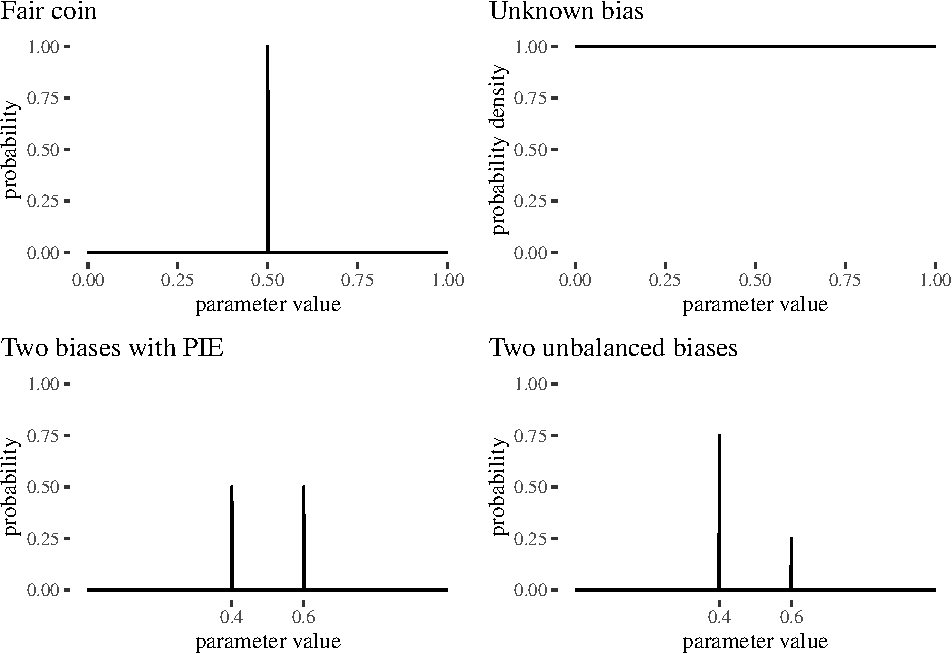
\includegraphics[width=1\linewidth]{impreciseEpistemicFINAL_files/figure-latex/fig:evidenceResponse-1} \end{center}
\caption{Examples of RA's distributions responding to various types of evidence for typical cases brought up in the literature.}


\label{fig:evidenceResponse}
\end{figure}

Perhaps, one might complain that now it is hard to distinguish between
(Two biases) in which nothing is known about the (higher-order)
probabilities of parameter values .4 and .6, and the case in which it is
known that these parameters have equal probability. This, however, would
be a complaint about the principle of insufficient evidence (PIE), not
about the representation itself. From the perspective taken here, more
can be done to take this uncertainty seriously. RA, for instance, could
in such a case deny that their stance could be summarized by a single
higher-order probability measure, but rather as a uniform distribution
over possible probabilities assigned to ``\(\mathsf{P(p) = .4}\)''
itself. At least in principle, it's turtles all the way up. How far we
go up the hierarchy depends on the trade-offs between practical
considerations, modeling complexity, and how much attention one wishes
to pay to various levels of uncertainty.

\hypertarget{qualitative-considerations}{%
\subsection{Qualitative
considerations}\label{qualitative-considerations}}

Summaries of RA's distributions are exactly that: a simplified and
therefore somewhat inadequate representations of the underlying
uncertainty. However, for some purposes---when simplification is
desirable and brings no serious harm---they might be useful.

One summary that comes in handy in the context of Bayesian statistics is
the highest density interval (HDI). It is the narrowest interval
containing a specified probability mass. HDIs are to be contrasted with
credible intervals, which span between \(\nicefrac{\alpha}{2}\) and
\(1-\nicefrac{\alpha}{2}\) quantiles of the probability mass. The key
difference is that credible intervals symmetrically get rid of tails of
a distribution, which might make sense if the distribution is fairly
symmetrical, but fails to be intuitive in other cases. To appreciate the
superiority of HDI in such contexts, take a look at Figure
\ref{fig:HPDIs} containing examples of comparisons of .5 HDIs with .5
credible intervals for two somewhat unusual distributions.

\begin{figure}

\begin{center}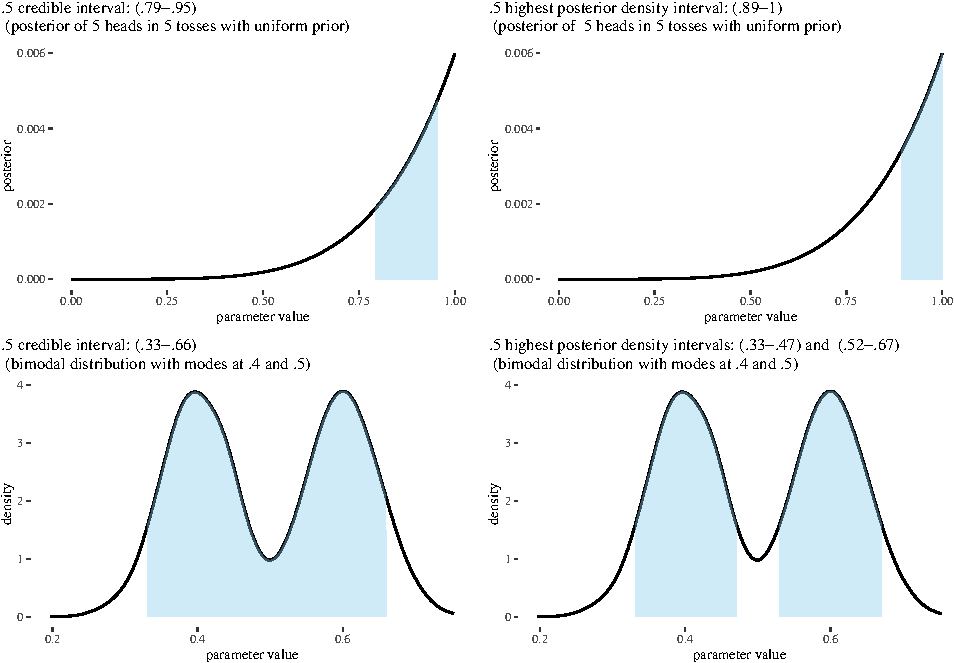
\includegraphics[width=1\linewidth]{impreciseEpistemicFINAL_files/figure-latex/fig:HPDIplot-1} \end{center}
\caption{Credible intervals vs. highest posterior density intervals illustrated on two unusual distributions.}
\label{fig:HPDIs}
\end{figure}

In the example, we used .5 HDIs and CIs, but often it is more sensible
to use a higher value, so we'll be using 89\%. The 89\% HDI includes all
those values of \(x\) for which the density is at least as large as some
value \(v\), such that the integral over all those \(x\) values is 89\%.

Some caveats. Note that the definition entails that the 89\% HDI of the
uniform distribution does not exist. For all \(v<1\) there are no values
of \(x\) such that \(p(x)>v\), and for \(v>=1\) all values of \(x\)
satisfy the condition and the integral is 1. For this degenerate case,
we will take the HDI to be the widest possible, \([0,1]\). Similarly, it
doesn't make much sense to talk about HDI if instead of a density
function we're dealing with a probability measure which assigns 0 to all
but finitely many points for whose probabilities sum to 1. Such a
measure is bounded, defined everywhere and the set of discontinuities is
of Lebesgue measure zero (that is, the function is piece-wise
continuous)--- so in principle we could integrate, the results aren't
exciting, as the integral 0 whatever the non-zero points are. For such
cases we will abuse the notation and say that the HDI starts at the
least non-zero \(x\) and ends at the largest non-zero \(x\). Notice also
that RA in reality is almost never in a situation where such a
probability measure is appropriate: even if they hold a real coin meant
to be fair, given various sources of errors in production it is simply
inappropriate to think that the chance of it being fair is exactly .5,
instead of using some probability density highly concentrated around
that value.

Now, here's one way RA might want to run their qualitative comparisons.
Suppose RA's HDIs for probability parameters \(a\) and \(b\) associated
with propositions \(A\) and \(B\) respectively have limits
\(a_l, a_h, b_l, b_h\) (\(a\) low, \(a\) high, \dots) respectively. We
can say that RA definitely considers \(A\) at least as likely as \(B\)
(\(A\geq B\)) just in case \(a_l\geq b_l\) and \(a_h \geq b_h\), that
\(A>B\) iff \(A\geq B\) but not \(B \geq A\), and that RA considers
\(A\) plausible just in case \(a_l>t\) for some sensibly high threshold
\(t\). This allows for clear-cut cases, but also for cases in which RA
is undecided, either about a comparison or about the plausibility a
single proposition.

For example, imagine a case in which RA's density and HDI for heads in a
continuous variant of unknown bias (\(H_u\)) is as illustrated in the
lower-right part of Figure \ref{fig:HPDIs}, as contrasted, say with a
unimodal density if the bias is known (\(H_k\)), concentrated around .5
with HDI \((.46,.54)\). On our approach, \(H_u \not \geq H_k\) and
\(H_k \not \geq H_u\), which is quite intuitive. If, instead, say we
were dealing with a known bias concentrated around .6 with HDI
\((.53,.67)\) (so the upper bound would be the same as in the bimodal
case), it would already be the case that \(H_k> H_u\), which also seems
intuitive.

Let's see how this approach handles Rinard's GREEN-MYSTERY argument
against the supervaluationist approach to qualitative comparison in IP.
Now we're looking at HDIs. For the GREEN urn, the HDI is just
\(g=[1,1]\), and since the distribution is uniform for the MYSTERY urn,
its corresponding HDI is \(m = [0,1]\). In this setting, clearly
\(g_l> m_l\) and \(g_h \geq m_h\), and so \(G\geq M\), but not
\(M\geq G\), and therefore \(G>M\). That is, RA, is more convinced about
\(G\) than they are about \(M\), as desired.

\hypertarget{intermezzo-entropy-and-divergence}{%
\subsection{Intermezzo: entropy and
divergence}\label{intermezzo-entropy-and-divergence}}

In what follows I will construct an information-theoretic inaccuracy
measure, and explicate the notion of evidential weight in
information-theoretic terms. For this reason, to make the paper fairly
self-contained and accessible, let me explain the key notions used in
what follows: entropy and divergence. While these are known to many
formal philosophers, there are some caveats to how I deploy them, and I
think the intuitive motivations for using them are worth rehearsing.

Let's start with a fairly simple binary case. Suppose you want to
navigate from \(A\) to \(D\), with the uninformed prior, at each
junction thinking that each choice is equally likely to be the right
one, your choices are visualized in Figure \ref{fig:entDAG}.

\begin{figure}[H]

\begin{center}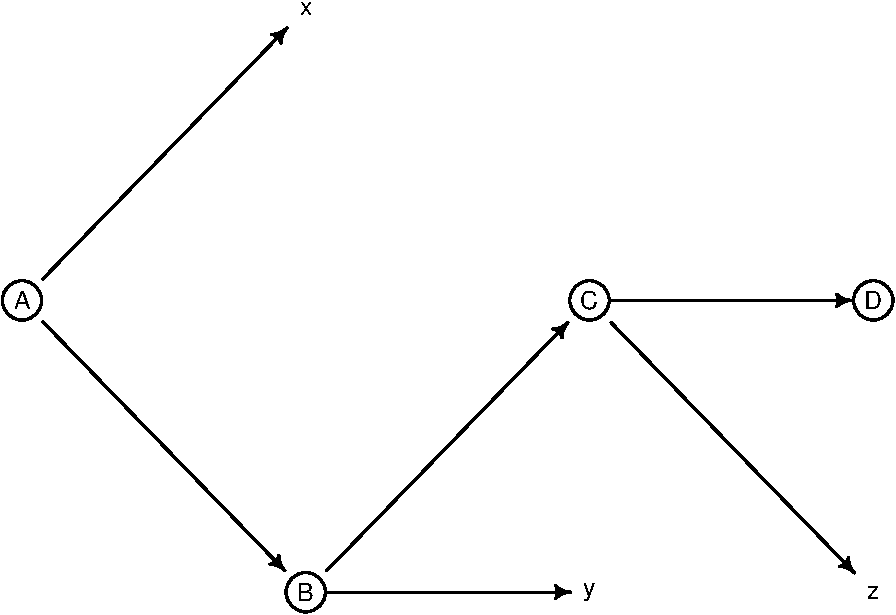
\includegraphics[width=0.7\linewidth]{impreciseEpistemicFINAL_files/figure-latex/label-1} \end{center}
\caption{You want to navigate from $A$ to $D$ with the uninformed prior.}
\label{fig:entDAG}
\end{figure}

I could describe the route to you using three digits. Suppose at each
point the path on the left is marked 1, and the one on the right is
marked 0. The right path is then 011. There are \(m=8\) possible
destinations that could be reached by making decisions at
\(\log_2(8)=3\) forks.

How much information are you given if I just tell you to take path 0 at
the first fork? Initially, you thought the probability that it is the
right one was .5. Now you know it is the right one. One natural measure
is \emph{surprise}, \(\nicefrac{1}{.5}=2\): there is a sense in which
you now have twice the information that you had. If to make sure your
measure of information is also additive, you transform surprise
logarithmically, the \emph{Shannon information} is
\(\log_2(\nicefrac{1}{.5})=1\). That is, you receive one \emph{bit} of
information. If you receive the complete instructions, assuming your
probabilities were independent, you receive
\(\log_2(\nicefrac{1}{.5^3})=3\). Thus, intuitively, Shannon's
information tracks the information you received in terms of how many
binary decisions you are now able to make assuming you initially thought
they were equally likely and independent. Further, notice that
\(\log_2(\frac{1}{a})= - \log_2(a)\) in general, so the official
definition of Shannon information goes: \begin{align*}
h(x) & = - \log_2 \mathsf{\pr{x}}
\end{align*} If the outcomes are equally likely, \(h(x)\) doesn't depend
on the choice of \(x\). However, if the distribution is not uniform,
this will not be the case. As a measure of (lack of) information
contained in a whole distribution, we use \emph{entropy} which is the
average Shannon information: \begin{align*}
H(X)  & = \sum \mathsf{P}(x_i) \log_2 \frac{1}{\mathsf{P}(x_i)} =
- \sum \mathsf{P}(x_i) \log_2 \mathsf{P}(x_i)
\end{align*} \noindent Note that entropy is not the measure of
information contained in a distribution. It is rather the opposite: the
expected amount of information you receive once you learn what the value
of \(X\) is. The less informative a distribution is, the more you expect
to learn when you find out the value of \(X\), the higher the entropy.
Also, not that entropy is the function of the measure itself, so
normally it makes sense to talk about the entropy of distributions
rather than variables.

Interestingly, the move to continuous distributions is not
straightforward. One might expect that it could be made by binning ad
taking the limit. For instance, suppose we divide \(X\) into bins
\(x_i\) of length \(\Delta\), so that we discretize \(X\) into
\(X^\Delta\). The discrete case definition applies: \begin{align*}
H(X^\Delta) & = \sum \left[\mathsf{P}(X \mbox{ is in the $i$-th bin}) \log_2 \frac{1}{\mathsf{P}(X \mbox{ is in the $i$-th bin})}\right]
\end{align*} \noindent If you think of the histogram of the distribution
of \(X^\Delta\) with total area \(A\), each bin has area \(a_i\) and
height \(p_i\). Suppose we normalize so that \(A =1\), then the
probability of each bin is \(\mathsf{P}_i = p_i \Delta\) and \(p_i\) can
be thought of probability density. Then we have: \begin{align*}
H(X^\Delta) & = \sum \mathsf{P}_i \log_2 \frac{1}{\mathsf{P}_i}\\
& = \sum p_i \Delta \log_2 \frac{1}{p_i \Delta}\\
& = \sum \left[ p_i \Delta \left(\log_2 \frac{1}{p_i} + \log_2\frac{1}{\Delta}\right)\right]\\
& = \sum p_i \Delta \log_2 \frac{1}{p_i} +    \underbrace{\sum \underbrace{p_i \Delta}_{\mathsf{P}_i}}_1 \log_2\frac{1}{\Delta} \\
& = \sum p_i \Delta \log_2 \frac{1}{p_i} +  \log_2\frac{1}{\Delta}
\end{align*} \noindent Accordingly, when we try to go continuous by
taking the limit, we get: \begin{align*}
H(X) & = \left[\int_{-\infty}^\infty p(x) \log_2 \frac{1}{p(x)}\, dx  \right] + \infty
\end{align*} \noindent This is, come to think of it, as it should: the
entropy of a continuous variable increases with the precision of
measurement, so infinite precision gives infinite information. For this
reason, for the continuous case it usual to drop the rightmost part of
the equation and talk about \emph{differential entropy}: \begin{align*}
H(X) & = \left[\int_{-\infty}^\infty p(x) \log_2 \frac{1}{p(x)}\, dx  \right] 
\end{align*} While in principle this is a fine tool, in what follows we
prefer to stick to entropy proper. One reason is that we will want to
meaningfully compare information conveyed by discrete distributions to
that conveyed by continuous ones. A convenient way to do so is to
abandon the idea that we should be infinitely precise, fix a certain
number of bins and keep it fixed in our comparison. This is what we will
do: effectively, we will be using \emph{grid approximations} of
continuous distributions: we will split \(X\) into a 1000 bins and use
the normalized densities for their centers to obtain their corresponding
probabilities. As long as we don't change our level of precision (which
would inevitably lead to changes in entropy) in our comparisons, this is
not a problem. An additional advantage is that now we don't have to deal
with the intricacies of explicit analytic calculations for continuous
variables and comparing apples (entropy) with oranges (differential
entropy).

Let's move forward towards a way to measure differences between
distributions. First, the notion of \emph{cross-entropy}. Suppose events
arise according to a distribution \(\mathsf{P}\) but we predict them
using a distribution \(\mathsf{Q}\). The \emph{cross-entropy} in such a
situation is \begin{align*}
H(\mathsf{P}, \mathsf{Q}) & = \sum \mathsf{P}_i \log_2(\mathsf{Q}_i)
\end{align*} This value is going to be higher than the entropy of
\(\mathsf{P}\) itself, if \(\mathsf{Q}\) is different from
\(\mathsf{P}\).\footnote{This claim will be important for the considerations of propriety and we will get around to proving it soon.}
Now think about the additional entropy introduced by using
\(\mathsf{Q}\) instead of \(\mathsf{P}\) itself, called
\emph{Kullback-Leibler divergence} (KL divergence): \begin{align*}
DKL(\mathsf{P}, \mathsf{Q}) & = H(\mathsf{P}, \mathsf{Q}) - H(\mathsf{P})\\
&= - \sum \mathsf{P}_i \log_2(\mathsf{Q}_i)  - \left(   - \sum \mathsf{P}_i \log_2 \mathsf{P}_i\right) \\
& = - \sum \mathsf{P}_i\left( \log_2 \mathsf{Q}_i - \log_2\mathsf{P}_i\right)\\
& =  \sum \mathsf{P}_i\left( \log_2 \mathsf{P}_i - \log_2\mathsf{Q}_i\right)\\
& = \sum \mathsf{P}_i \log_2 \left( \frac{\mathsf{P}_i}{\mathsf{Q_i}}\right)
\end{align*} \noindent  That is, KL divergence is the expected
difference in log probabilities. In particular, if
\(\mathsf{P}=\mathsf{Q}\) we get
\(DKL(\mathsf{P},\mathsf{P}) = \sum \mathsf{P}_i (\log_2 \mathsf{P}_i - \log_2 \mathsf{P}_i) = 0\),
which works out as it intuitively should
be.\footnote{Note that often the natural logarithm function is used in the divergence calculations; this only is a shift of scale and doesn't make much difference.}

\hypertarget{weight-of-evidence}{%
\subsection{Weight of evidence}\label{weight-of-evidence}}

There is no agreed-upon list of desiderata on the notion of weight of
evidence, but presumably, these ideas look plausible:

\begin{enumerate}
\item Items of evidence leading to different expected values should be able to have the same weight.
\item Items of evidence leading to the same value should be able to have different weights.
\item In simple set up, such as Bernoulli trials, weight should increase with the number of observations.
\item For unimodal distributions, the wider the distribution associated with a given piece of evidence, the less weight this evidence has.
\end{enumerate}

Now let's see how the conceptual tools introduced in the previous
section can help us explicate the notion of weight in a fairly
principled manner. First, the desiderata mention distributions, but
which ones do we mean? Clearly, we should not simply mean the posterior
distribution, as it is shaped not only by the evidence but also by the
priors. Perhaps, it makes sense to compare the posterior with the
prior---but then, one needs to remember that the result might be
sensitive to the prior, and it is not clear that the notion of weight of
evidence should be. Another would be to think of weights as assigned to
likelihood functions, but this comes with some caveats. Our approach
will be modular. First, we'll talk of weights as associated with
distributions. In this sense, if you think it makes sense to talk about
weights of evidence in terms of how uneven the posterior is, compared to
the prior, be my guest. In this wide sense, weights are just transformed
distances from uniform distributions, giving us an information-theoretic
measure of how uneven a distribution is. Once we go over this, I will
gesture towards a method of implementing this approach to likelihoods.

The idea is that the more informative a piece of evidence is, as
compared to the uniform distribution, the more weight it has, on scale 0
to 1: if the drop from uncertainty is complete, the entropy drops to
zero, and we would like the weight to be 1, if the drop is null we would
like to be zero, and if the drop is half, we would like to be .5 (and so
on for other proportions). This can be achieved by the following
definition: \begin{align*}
\mathsf{w(P_i)} & = 1 - \left( \frac{H(\mathsf{P})}{H(\mathsf{uniform})}\right)
\end{align*} \noindent where \(\mathsf{P}\) is the discrete probability
distribution for a given number of bins \(n\), and uniform is the
discrete uniform distribution for the same number of
bins.\footnote{In some contexts it might make sense to measure improvement with respect to a non-uniform prior. In such cases,  $H(\mathsf{uniform})$ is to be replaced by $H(\mathsf{prior})$.}
Note that the entropy of a uniform distribution is pretty
straightforward, so we can simplify: \begin{align*}
H(\mathsf{uniform}) & = \sum_{i=1}^n \nicefrac{1}{n} \log_2 \frac{1}{\nicefrac{1}{n}} \\
& = \log_2(n) \\
\mathsf{w(P_i)} & = 1 - \left( \frac{H(\mathsf{P})}{\log_2(n)}\right)
\end{align*}

Let's first see how this plays out with beta distributions. The
advantage of looking at them first is that they have a fairly
straightforward interpretation: \(\mathsf{beta(a,b)}\) is the
distribution one should have when tossing a coin with unknown bias,
having observed (or imagining to have observed) \(a\) heads and \(b\)
tails, imagining that seeing one heads and one tails leaves you
uninformed. From this perspective, \(\mathsf{beta(1,1)}\) is the uniform
distribution, \(\mathsf{beta(40,10)}\) is the likelihood corresponding
to 40 heads and 10 tails, and so on. To get a feel for what beta
distributions look like, inspect Figure \ref{fig:betas}. Remember we're
working with a grid approximation (\(n=1k\)).

\begin{figure}[H]


\begin{center}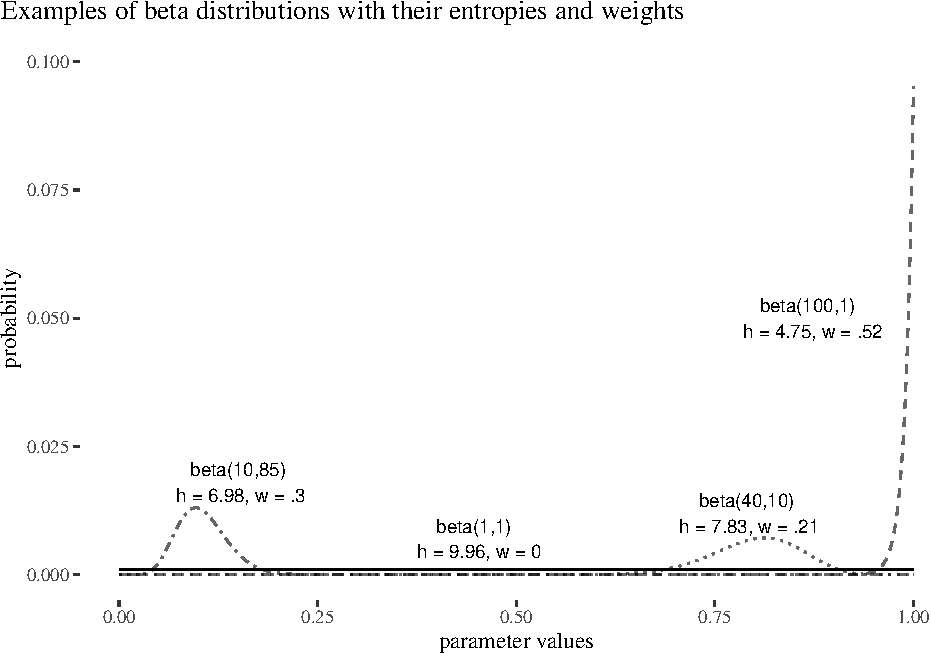
\includegraphics[width=1\linewidth]{impreciseEpistemicFINAL_files/figure-latex/fig:betas3-1} \end{center}
\caption{Examples of beta distributions with entropies and KL divergencies from the uniform distribution with grid approximation ($n=1000$). Note that distribution weight does not strongly depend on its expected value.}
\label{fig:betas}
\end{figure}

Now, consider a whole range of beta distributions for all combination of
integers from 1 to 100 used as \(a\) and \(b\). Their entropies are
visualized in Figure \ref{fig:entropies}.

\begin{figure}[H]

\begin{center}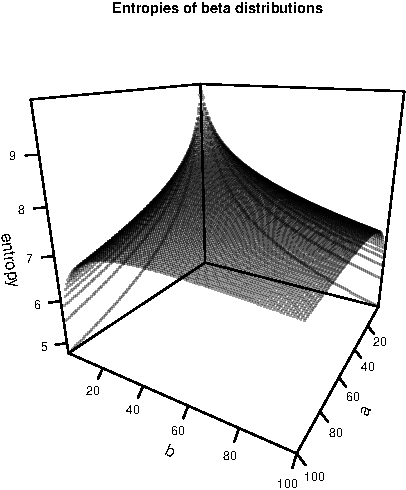
\includegraphics[width=1\linewidth]{impreciseEpistemicFINAL_files/figure-latex/fig:entropies-1} \end{center}
\caption{Entropies of beta distributions for a and b ranging from 1 to 100. Entropy decreases as they increase.}
\label{fig:entropies}
\end{figure}

Two phenomena are as expected. First, the entropy decreases with the
number of observations, and second, it decreases faster if the
proportions are closer to the extremes. This is mirrored by the
corresponding weights (Figure \ref{fig:weights}).

\begin{figure}[H]

\begin{center}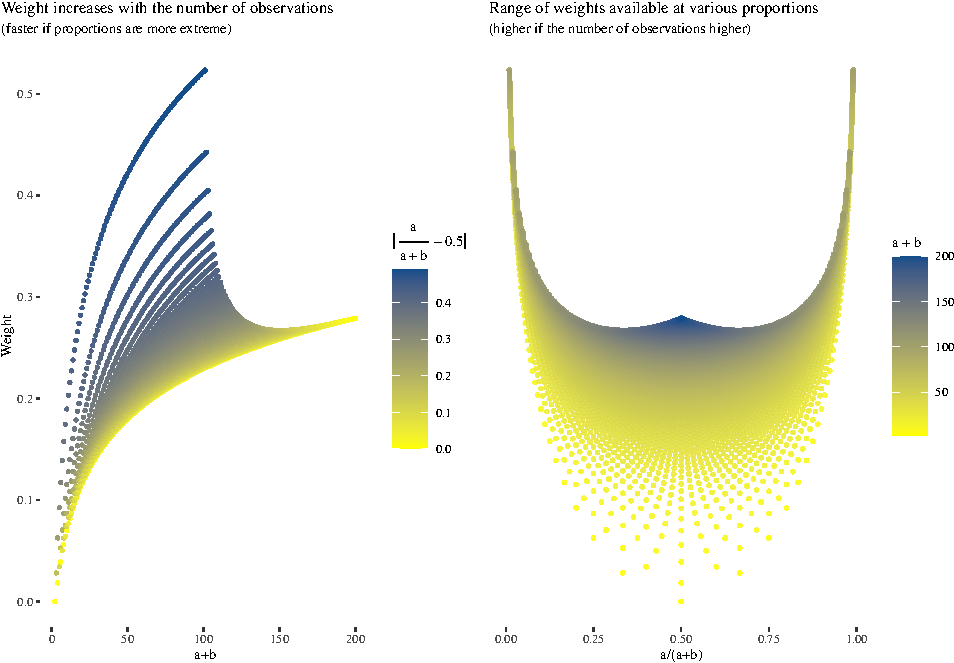
\includegraphics[width=1\linewidth]{impreciseEpistemicFINAL_files/figure-latex/fig:weights-1} \end{center}
\caption{Weights of beta likelihoods for $a,b$ ranging from $0$ to $100$, versus the number of observations   and versus absolute distance of the proportion from .5.}
\label{fig:weights}
\end{figure}

Now, let's see whether the results are intuitive for comparisons of
distributions of various shapes, including those involving all weights
focused on a particular point (strictly speaking, a single bin in the
grid approximation). So here's a selection of shapes worth looking at
(Figure \ref{fig:weightsWeird}).

\begin{figure}[H]

\begin{center}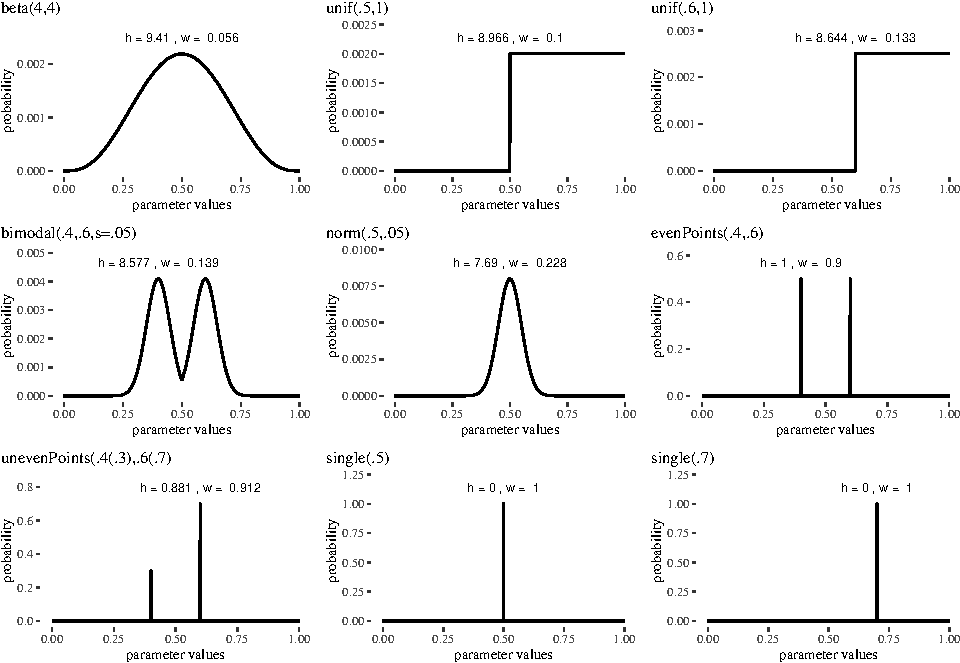
\includegraphics[width=1\linewidth]{impreciseEpistemicFINAL_files/figure-latex/fig:weightsWeird-1} \end{center}
\caption{Examples of various distributions with their entropies and weights, ordered by weights. (1) beta(4,4), (2) uniform starting from .5 to 1, (3), uniform strating from .6 to 1, (4) two normal distributions centered around .4 and .6 with standard deviation .05, glued at .5. (5) normal centered around .5 with the same standard deviation, (6) one that assigns .5 to each of .4  and .6, (7) One that assigns .3 to .4 and .7 to .6., (8) one that assigns all weight to .5, and (9) one that assigns all weight to .7.}

\label{fig:weightsWeird}
\end{figure}

Note that the ordering of weights is as expected. Partial uniform
likelihoods which exclude at least half of parameter values have more
weight than a weak beta, and the weight increases as the non-zero
interval of the partial uniform distribution decreases. A bimodal normal
distribution ``glued'' from two normal distributions carries less weight
than a unimodal normal distribution with the same standard deviation
centered around the mean of the two modes, all these are way below point
estimates. If multiple points have non-zero probability, the weight
depends on how uneven the distribution is, whereas if full weight is
given to a single point, the value of the parameter is known, the weight
is maximal (=1) and does not depend on what the parameter is.

Right, but how we apply the notion of weight to evidence? Crucially, the
weight of evidence is captured in precise contexts by likelihood ratios,
and in the standard Bayesian contexts by likelihood functions. A
likelihood ratio of a piece of evidence \(E\) with respect to a
hypothesis \(H\) is the ratio of two probabilities: the conditional
probability of the evidence given the hypothesis, and the conditional
probability of the evidence given its negation,
\(\nicefrac{\pr{E \vert H}}{\pr{E \vert \n H}}\). For instance, suppose
that you learn that if a child has been the victim of abuse, the
probability that they will have the habit of rocking is .3. How strong
is the evidence when you observe a given child rocks? Well, this depends
on how probable rocking is given that the child has not been abused. The
likelihood ratio accounts for both elements in its evaluation of the
evidence.

A likelihood function, on the other hand, assigns probability of the
data to each particular parameter value,
\(l(\theta) = p(E\vert \theta)\). Our formal setup requires likelihood
functions, so it would be useful to have a way of accommodating cases in
which point estimates (and so the usual likelihood ratios) are
available. One way to go about this is to take expected values:
\(\pr{E\vert \theta} = \pr{E \vert H} \theta + \pr{E \vert \n H}(1- \theta)\).
Coming back to our example, if the probability of rocking conditional on
abuse is .3, and it is .1 conditional on lack thereof, the likelihood
will reach .3 for \(\theta =1\), go down to \(1\) at \(\theta = 0\), and
go linearly between these extrema for the intermediate values of
\(\theta\).

Notably, likelihood function does not have to intergrate (or sum, in the
case of grid approximations) to 1. For instance, if the probability of
the evidence is .8 no matter what \(\theta\) is, the sum will be \(.8n\)
for \(n\) bins. Note that flat likelihoods like that, intuitively, are
not informative with respect to the relevant hypotheses---they provide
no guidance as to \(\theta\), and it doesn't matter at what value they
fall flat. For this reason, and to make the weight calculations
comparable, I propose that likelihoods first should be normalized to
integrate/sum to 1, and then we should use the notion of weight we
already introduced. To see how this works out, let's continue with the
rocking example.

Suppose you are slightly but vaguely suspicious, starting with
\(\mathsf{beta}(2,4)\) prior (dashed in the figure below). Your original
89\% HDI is (.052,.6). Now imagine two scenarios. In both you learn that
the child rocks, but in the first you start with a linear likelihood
function going from \(.1\) to \(.3\), and in the other the likelihood
goes from \(.001\) to \(.95\). The likelihoods and the corresponding
shifts in the posteriors and the HDIs are visualized in Figure
\ref{fig:likelihood}. In each case, rocking, unsurprisingly, turns out
to be insufficient evidence, even given that you started with some
suspicion, but the impact of the evidence on the posteriors is
different.

\begin{figure}[H]

\begin{center}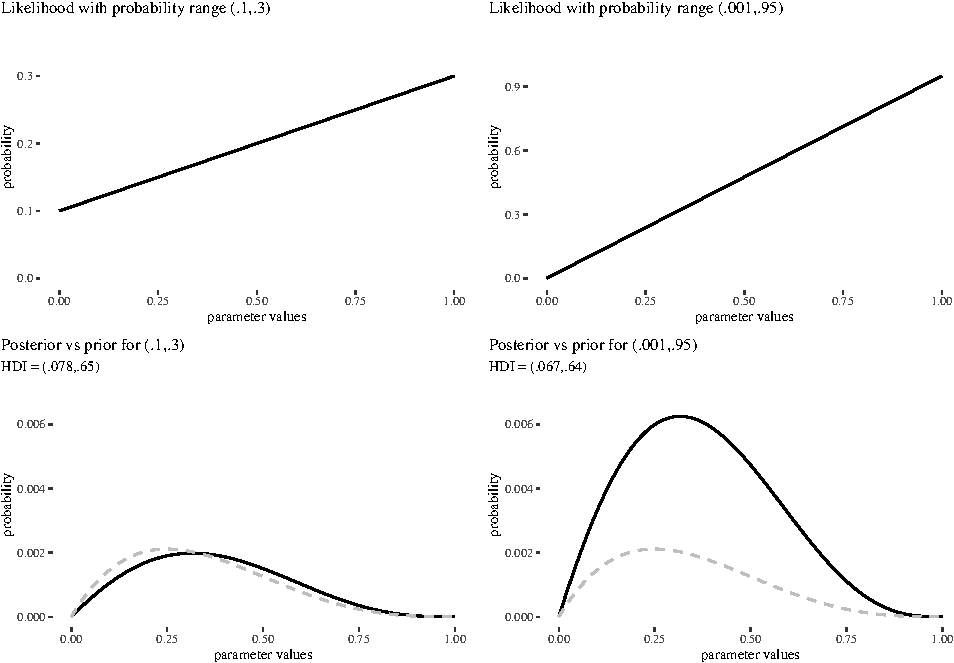
\includegraphics[width=1\linewidth]{impreciseEpistemicFINAL_files/figure-latex/fig:likelihood-1} \end{center}
\caption{Impact of evidence with linear likelihood based on point estimates. Prior marked with dashed line.}
\label{fig:likelihood}
\end{figure}

Weights of normalized likelihoods are \(.006\) (left) and \(0.2\)
(right), which captures the intuition that the second item of evidence
is much stronger. Notice also that while the weight of the prior is
\(0.052\), the posterior weights are not much different, \(.046\)
(left), and \(0.049\) (right). This is because there is a sense your
evidence made you more uncertain, as your posterior distributions'
centers are closer to the middle. The lesson here is that the weights of
posterior distributions might not be a good guide to weights of
particular items of evidence, and that the framework can capture cases
in which obtaining new evidence might make you more confused (albeit,
perhaps, closer to the true). If needed, one can measure the change of
weight between the prior and the posterior in terms of the difference
between weights of the prior and the posterior, or the absolute value
thereof. What if no precise likelihood is available? Then, higher-order
densities about \(\pr{E \vert H}\) and \(\pr{E\vert \n H}\) will result
in a density over potential likelihood ratios.

Now that we have at least a promising candidate for an explication of
the notion of weight of evidence, let's turn to belief inertia and see
how it can be handled from the higher-order perspective.

\hypertarget{belief-inertia-1}{%
\subsection{Belief inertia}\label{belief-inertia-1}}

In contrast with what happens if you start with the set of all possible
representors, here the learning is fairly easy to model. If you just
start with a uniform density over \([0,1]\) as your prior, use binomial
probability as likelihood, observing any non-zero number of heads will
exclude 0 and observing any non-zero number of tails will exclude 1 from
the basis of the posterior. Let's see an example with a grid
approximation (\(n=1k\)). For simplicity assume there are only green and
black balls. Our prior is uniform, and then, in subsequent steps, we
observe one green ball, another green ball, and then a black ball. This
is what happens with the posterior as we go (Figure
\ref{fig:intertia2}).

\begin{figure}[H]

\begin{center}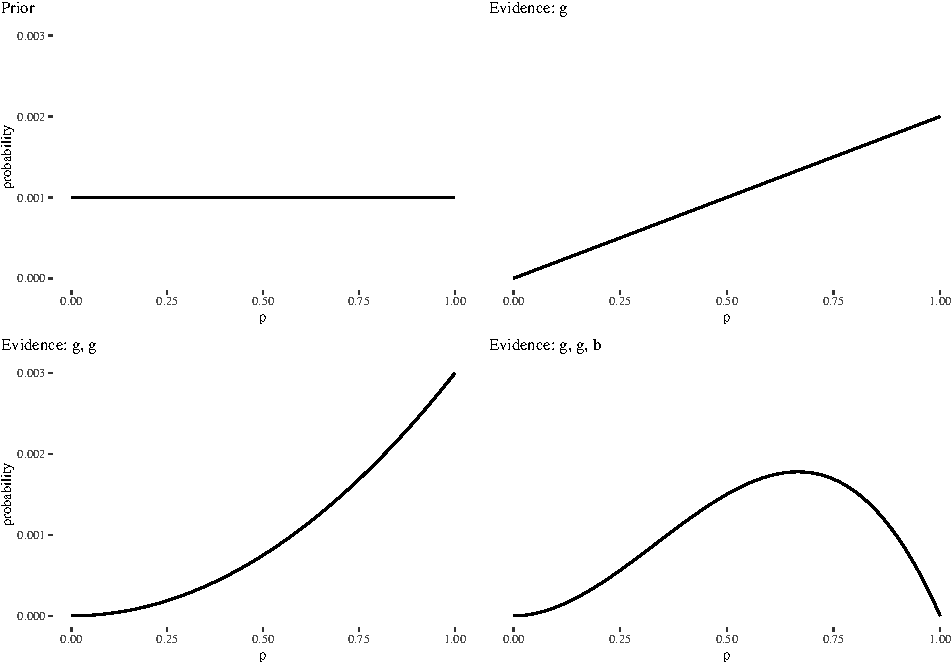
\includegraphics[width=1\linewidth]{impreciseEpistemicFINAL_files/figure-latex/fig:inertia2-1} \end{center}
\caption{As observations of green, green and black come in, extreme parameter values drop out of the picture and the posterior is shaped by the evidence.}
\label{fig:intertia2}
\end{figure}

To see how this approach is also capable of modeling Rinard's example of
inertia, lets start with MaxEnt recommending even priors of the two
chance hypotheses. In Figure 10 we see what usual calculations revise
these priors to, as we obtain new evidence, again, say: green, green,
black. This behaves completely as expected with no inertia in sight.
Note how the observations initially support \(H_1\), but exclude \(H_1\)
in the last stage.

\begin{center}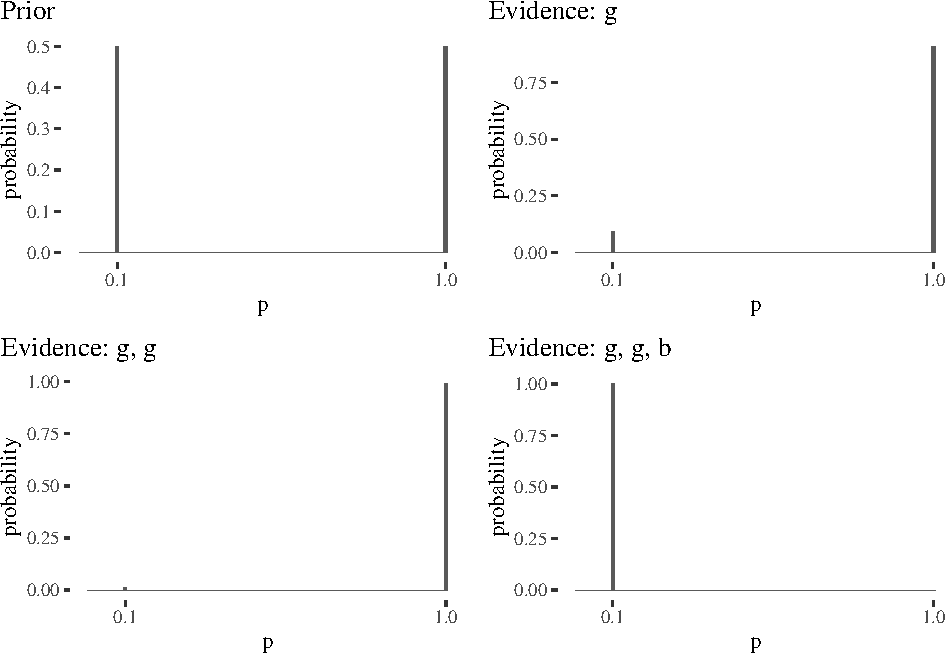
\includegraphics[width=1\linewidth]{impreciseEpistemicFINAL_files/figure-latex/rinardCalculations-1} \end{center}

\begin{figure}[H]

\caption{Learning in Rinard's example of belief inertia.}
\label{fig:rinard2}
\end{figure}

\hypertarget{accuracy-1}{%
\subsection{Accuracy}\label{accuracy-1}}

Now, let's turn to accuracy. While the imprecisers have hard time
defining what the accuracy of a set of measures is, our path is easier.
Already some work has been done on the notion of accuracy of continuous
probability distributions. One key notion in use is that of continuous
ranked probability score (CRPS) of a distribution \(p\) with respect to
a possible world \(w\): \begin{align*}
I(p,w) &= \int_{-\infty}^\infty \vert \mathsf{P}(x) - \mathbf{ 1 }(x\geq V(w))\vert ^2 \, dx
\end{align*} \noindent where \(\mathsf{P}\) is the cumulative
probability corresponding to a given density, and \begin{align*}
\mathbf{ 1 }(x \geq V(w)) & = \begin{cases} 1 & \text{ if } x \geq V(w)\\
0 & \text{ o$\,$/w. }
\end{cases}
\end{align*} \noindent  The intuition here is that the measure takes the
Cramer-Von-Mises measure of distance between densities, defined in terms
of the area under the squared euclidean distances between the
corresponding cumulative density functions: \begin{align*}
\mathcal{C}(p,q) & = \int_{0}^{1} \vert P(x) - Q(x)\vert^2 \, dx
\end{align*} \noindent and uses it to measure distance to an
epistemically omniscient chance hypothesis, which either puts full
weight on 0, if a given proposition is false, or on 1, otherwise. We
will start building by reflecting on this approach.

First, as in practice we are unable to work with infinite precision
anyway, not much harm is done and much computational ease is made with
(grid) approximations, so I will keep using these in line with the
previous developments (note for instance that there are no readily
computable solutions to the integral used in the definition of CRPS,
although it can sometimes be evaluated in closed form). So, instead of
integration, we'll be using summation over the values for a finite
number of bins.

Now, let's see how this approach would play out in a scenario very much
like Schoenfield's (EMC), with an additional layer of uncertainty: the
opponent will produce two coins, one with the distribution of Heads
either normal around \(.3\), and one normal around \(.5\), both with the
standard deviation of \(.05\), randomly pick one of these coins and then
toss it. The RA knows the setup. Consider the following three (out of
many) possible stances that RA could take:

\begin{figure}[H]

\begin{center}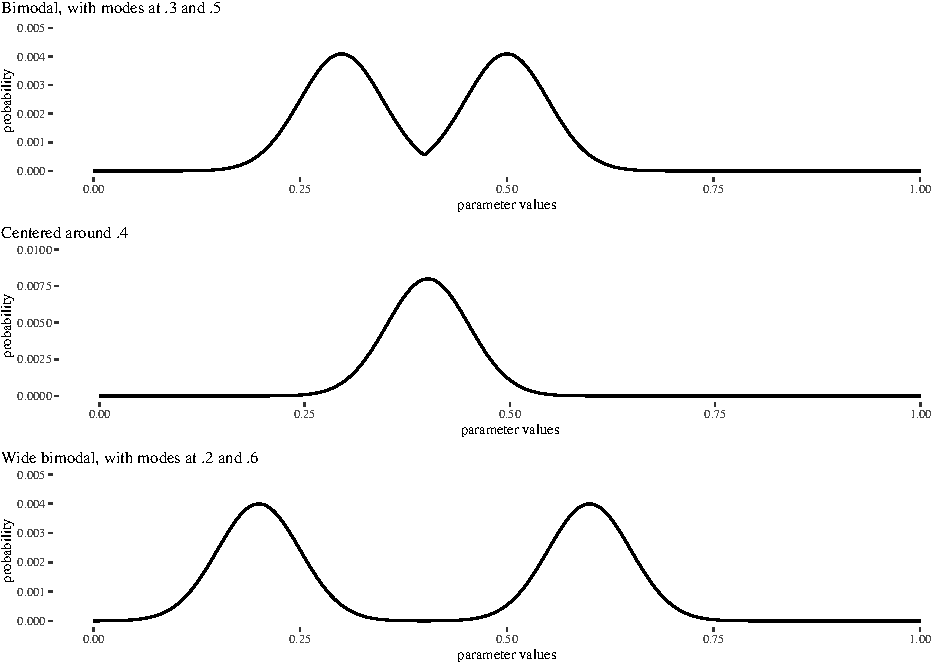
\includegraphics[width=1\linewidth]{impreciseEpistemicFINAL_files/figure-latex/figEMC-1} \end{center}
\caption{Three (out of many) candidates in a vague EMS scenario. All distributions are built from normal  distributions with standard deviation $.5$, the bimodal ones are "glued" in the middle.}
\label{fig:EMC}
\end{figure}

An impreciser might be inclined to say that it is the bimodal
distribution that's appropriately evidence-responsive. The centered one,
while centering on the expected value, definitely gets the chances
wrong, while the wide bimodal has its guesses too close to truth values
and too far from the actual known chances. Now, is this in any way
mirrored by CRPS and expected CRPS calculations? It turns out it isn't.

\begin{table}[H]
\centering
\begin{tabular}{lrrrrrr}
\toprule
distribution & CRPS1 & CRPS0 & KLD1 & KLD0 & ExpCRPS & ExpKLD\\
\midrule
bimodal & 534.7305 & 334.9305 & 80.06971 & 33.90347 & 414.8505 & 52.36997\\
centered & 571.2192 & 371.4192 & 110.84220 & 53.13440 & 451.3392 & 76.21752\\
wide bimodal & 485.4052 & 285.6177 & 54.13433 & 19.50965 & 365.5340 & 33.35974\\
\bottomrule
\end{tabular}
\caption{CPRS and KLD inaccuracies of the three distributions to the TRUE and FALSE omniscient functions, with expected inaccuracies.}
\end{table}

Notice that the expected inaccuracy recommend the wide bimodal
distribution, which does not seem desirable! This, notice also, doesn't
change if instead of CRPS we use the KL divergence from the omniscient
measure, so it doesn't seem like the choice of the measure itself is the
culprit here.

The problem here is that all these distributions have the same expected
value: \(.4\), which is used in the calculations of the expected
inaccuracies. This also means that not only the wide bimodal
distribution expects itself to be the least inaccurate, but also that
other measures expect it to be the least inaccurate! This also suggests
that the strategy of (i) calculating two distances/divergencies from the
two extreme omniscient measures and (ii) averaging by plugging in the
expected value, does not result in a proper inaccuracy score.

But this strategy is clearly against the spirit of our enterprise. If we
start with the idea that expected values are often not good
representations of RA's uncertainty, it is not terribly surprising that
they do not lead to sensible expected inaccuracy calculations. After
all, since the three distributions do have the same expected value, the
difference between the probabilities they assigned don't seem to be
taken seriously in the weighting stage (ii). The question now is, how
can we do justice to the complexity of RA's credal state in the expected
inaccuracy considerations?

Well, if we start with taking RA's higher order probabilities to be
probabilities about which parameter values are the right ones (true
chances, real population frequencies, the point credences justified by
the evidence, or what have you, philosophically speaking), we should see
how taking these intuitions seriously plays out. So, instead of
measuring inaccuracy with respect to two omniscient credences peaking at
either 0 or 1 and averaging using expected values, we should instead
look at \(n\) potential true probability hypotheses, each of them
pointed at a single bin in our approximation, calculate all the
inaccuracies with respect to their corresponding omniscient functions,
and calculate the expected inaccuracies scores using whole distributions
rather than their expected values.

For the three distributions we're discussing in this chapter, the
inaccuracies calculated using CRPS and KL divergence with respect to
various potential true probability distributions look as in Figure
\ref{fig:inaccuracies2}.

\begin{figure}[H]

\begin{center}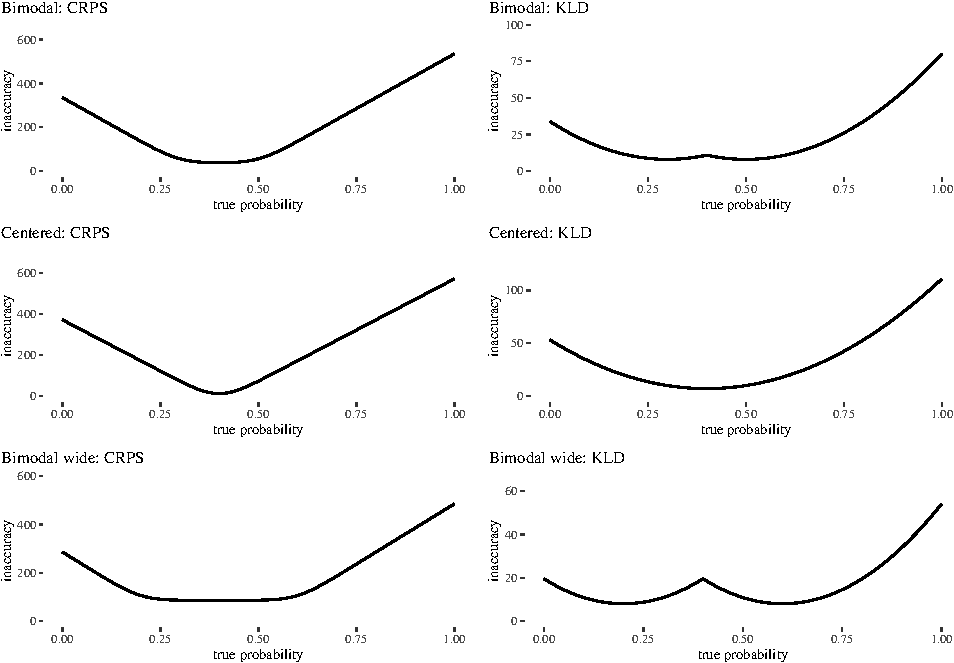
\includegraphics[width=1\linewidth]{impreciseEpistemicFINAL_files/figure-latex/fig:inaccuracies2-1} \end{center}
\caption{CLPSR and KL divergence based inaccuracies vs (omniscient functions corresponding to) $n$ true probability hypotheses for the three distributions discussed in this section.}
\label{fig:inaccuracies2}
\end{figure}

One important difference transpires between using CRPS rather than KLD.
Notice how for chance hypotheses between the actual peaks the inaccuracy
remains flat. This seems to be an artifice of choosing a squared
distance metric. If instead we go with a more principled,
information-theory-inspired KL divergence, inaccuracy in fact jumps a
bit for values in between the peaks for the bimodal distributions, which
seems intuitive and desirable.

Note that now the expected inaccuracies of the distributions from their
perspective look as in \mbox{Table \ref{tab:expected2}.}

\begin{table}[H]
\begin{tabular}{lrrrrrr}
& \multicolumn{3}{c}{CPRS} & \multicolumn{3}{c}{KLD} \\
\toprule
  & bimodal & centered & wide bimodal & bimodal & centered & wide bimodal\\
\midrule
bimodal & 64.670 & 78.145 & 88.380 & 8.577 & 10.655 & 11.336\\
centered & 41.657 & 28.181 & 85.911 & 9.239 & 7.690 & 15.627\\
wide bimodal & 137.699 & 171.719 & 113.989 & 11.541 & 19.231 & 8.689\\
\bottomrule
\end{tabular}
\caption{Expected inaccuracies of the three distributions from their own perspectives. Each row corresponds to a perspective.}
\label{tab:expected2}
\end{table}

Note that now the results are as intuitively they should: each
distribution recommends itself. How does the framework capture the idea
that it is the bimodal distribution that seems more adequate than the
others?

Well, one way to go would be to measure inaccuracy with respect to the
only chance hypotheses that should be on the table, given the
testimonial evidence. \(H_3\) on which the true chance is \(.3\) and
\(H_5\) on which the true chance is \(.5\). The respective inaccuracies
are as in Table \ref{tab:schoen}.

\begin{table}[H]
\begin{tabular}{lrrrr}
 & \multicolumn{2}{c}{CRPS} & \multicolumn{2}{c}{KLD} \\
\toprule
&H3 & H5 & H3 & H5\\
\midrule
bimodal &55.475 & 55.378 & 7.935 & 7.935\\
centered &72.281 & 72.090 & 9.836 & 9.825\\
wide bimodal & 86.230 & 86.223 & 10.871 & 10.882\\
\bottomrule
\end{tabular}
\caption{CRPS and KLD inacurracies of the three distributions with respect to the two hypotheses. Note that on both inaccuracy measures the bimodal distribution dominates the other two.}
\label{tab:schoen}
\end{table}

Just to double-check if some of this desirable outcome isn't caused by
not using pointed credences, we can run the calculations using the
pointy version: with all the weight on .4, or weights split in half,
either between \(.3\) and \(.5\), or between \(.2\) and \(.6\). As
expected, inaccuracy considerations recommend the bimodal version,
whichever of the two hypotheses holds (Table \ref{tab:schoen2}).

\begin{table}[H]
\begin{tabular}{lrrrr}
 & \multicolumn{2}{c}{CRPS} & \multicolumn{2}{c}{KLD} \\
\toprule
 &H3 & H5 & H3 & H5\\ \midrule
pointed bimodal &49.75 & 49.75 & 1.00 & 1.00\\
pointed centered &100.00 & 100.00 & 16.61 & 16.61\\
pointed wide bimodal & 99.75 & 99.75 & 16.61 & 16.61\\
\bottomrule
\end{tabular}
\caption{CRPS and KLD inacurracies of the three pointed distributions with respect to the two hypotheses.}
\label{tab:schoen2}
\end{table}

Now, the reader might worry that this has been only a discussion of an
example, which fails to establish the strict propriety of the KLD
inaccuracy measure. Fair point. In fact, such a proof is given in the
appendix to this paper. Just to get the gist of the argument, consider
taking the inaccuracy of a second-order discretized probability mass
\(p\) over a parameter space \([0,1]\), given that the real probability
is \(\theta\) as the Kullback-Leibler divergence of \(p\) from the
indicator distribution of \(\theta\) (which assigns 1 to \(\theta\) and
0 to all other parameter values in the parameter space), denoted as
\(\mathcal{I}_{\dkl}^2\).\footnote{The argument generalizes to parameter spaces that correspond to probabilities of multiple propositions which are Cartesian products of parameter spaces explicitly used in the argument in this section.}
It turns out that this is a strictly proper inaccuracy measure: each
\(p\) expects itself to be the least inaccurate distribution. The
argument has four key moves.

\begin{enumerate}
\item the inaccuracy of $p$ w.r.t. to parameter $\theta$ is just $- \log_2 p(\theta)$,
\item  the expected inaccuracy of $p$ from the perspective of $p$ is the entropy of $p$, $H(p)$,
\item  the inaccuracy of $q$ from the perspective of $p$ is the cross-entropy $H(p,q)$,
\item and it is an established result that cross-entropy is strictly larger than entropy as soon as $p\neq q$.
  \end{enumerate}

These are the points that are established in the appendix.

\hypertarget{pooling-and-synergy-1}{%
\subsection{Pooling and synergy}\label{pooling-and-synergy-1}}

How to go about opinion pooling from this perspective? First, let's
think about Gallow's example we've already described and suppose we
indeed want to employ linear averaging. Suppose you're considering two
experts, Al and Bert, and start with a uniform credal state. You think
the experts are way more competent than you---suppose your distribution
of trust is expressed by assigning weights \((.05,.6,.35)\) to you, Al,
and Bert, respectively. When you hear from Al only, you re-scale the
first two weights so that they add up to one and use them, and when you
hear from Bert only, you re-scale the first and the third weight and
plug these weights in your calculations. If you hear from both experts,
you use all three weights. An example of some potential results of this
procedure are visualized in Figure \ref{fig:gallow}.

\begin{figure}[H]

\begin{center}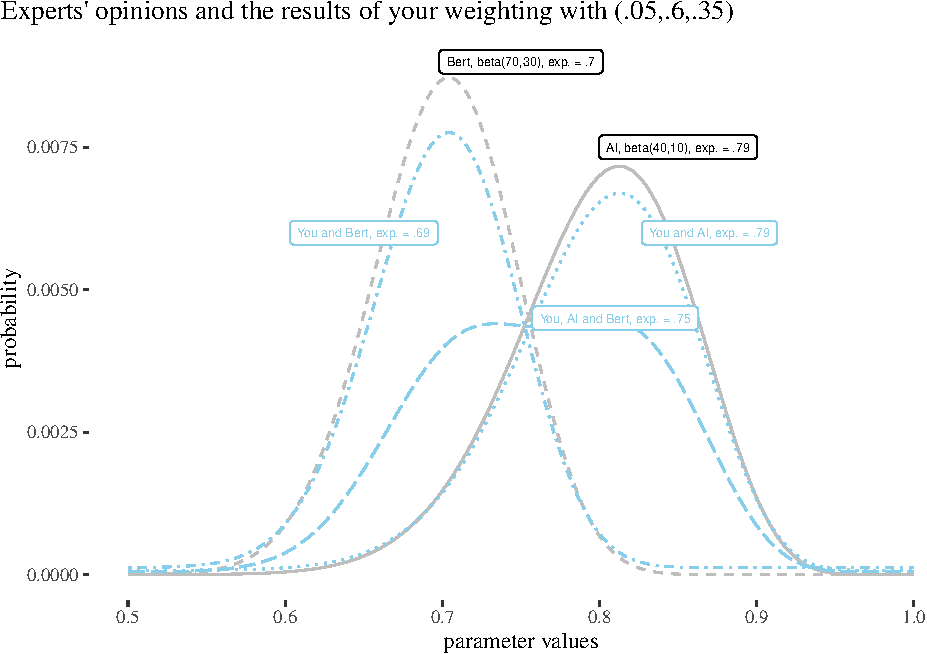
\includegraphics[width=1\linewidth]{impreciseEpistemicFINAL_files/figure-latex/fig:gallow-1} \end{center}
\caption{Linear pooling results for a Gallow-style situation.}
\label{fig:gallow}
\end{figure}

\noindent Reformulated for the current framework, one intuition behind
Gallow's postulates was that your expected probability given a single
expert's opinion should follow the expert's. While this idea of complete
deference to an expert has some tradition in the philosophical
literature, neither we nor current developments in formal epistemology
(Dorst, Levinstein, Salow, Husic, \& Fitelson, 2021) find it completely
plausible. If there is at least some reason to think the expert might be
mistaken, complete and absolute deterrence to the expert is too strong.
However, when our trust in the expert is quite strong an our prior
opinion fairly weak, the prior will only slightly dampen the expert's
opinion, not moving the expected value too much, and our posterior
should be very close to the expert's. We think that the fact that the
expected values of \textsf{You and Bert} and \textsf{You and Al} don't
shift much captures this intuition.

Another requirement was that in such a set-up, the revised opinion in
light of both experts' opinion should be the result of linear pooling of
some sort. Indeed, such pooling can be performed. Notice also that while
Al's opinion was weaker than Bert's, your revised opinion after hearing
both opinions has a more distinctive peak near to where Al's mode was,
which happened because you trusted Al almost twice as much as you
trusted Bert.

It is, however, by no means obvious that linear pooling is the best we
can do in circumstances of this kind. To illustrate, let's now get back
to the synergy example. This is an extreme simplification, but we'll use
it to make a conceptual point. Suppose you---Dr Alban---and the other
doctor, Dr Dre, starting from a uniform distribution have observed a
number of cases each, in which a treatment was provided to a patient,
and each of you recorded the number of observed successes. You assume
the individual cases were independent of each other and that the groups
you observed didn't differ in any relevant respect. You observed 97
successes out of 100 and so your posterior (having started with
\(\mathsf{beta}(1,1)\) is \(\mathsf{beta(98,4)}\). Dr Dre reports her
uncertainty as a \(\mathsf{beta(97,5)}\), having observed 96 out of 100
cases. What should your opinion be once you learn what Dr Dre believes?

Well, this certainly depends on how many observations are common to the
both of you. On one extreme, you were recording the same cases, and Dr
Dre also observed the same number of successes out of 100. She is a
unicorn a philosopher might call an \emph{epistemic peer}: she,
supposedly, is as capable as you, has exactly the same priors and
background, and observed exactly the same data. From our perspective,
though, if her inferential apparatus is the same, her formal model is
the same, she observed the same data, and yet revised to a different
distribution, she has made a mistake in her calculations, and the
appropriate distribution is exactly the one you already have. Moreover,
you should not learn anything from hearing her reports about the data
she observed, because you don't want to count the same data twice.

On another extreme, she observed a disjoint class of cases and did not
make a mistake. Then, it seems you should \emph{not} use linear pooling,
as now her report informs you that you jointly have observed 200 cases,
7 of which were failures. Thus, your revised credal state is better
captured by \(\mathsf{beta(194,8)}\). We'll call this latter method
\emph{expansion}. We also illustrate linear pooling the two opinions
(say, with you putting \(.7\) of trust in yourself and \(.3\) in Dr
Dre). The results are illustrated in Figure \ref{fig:dre}.

\begin{figure}[H]

\begin{center}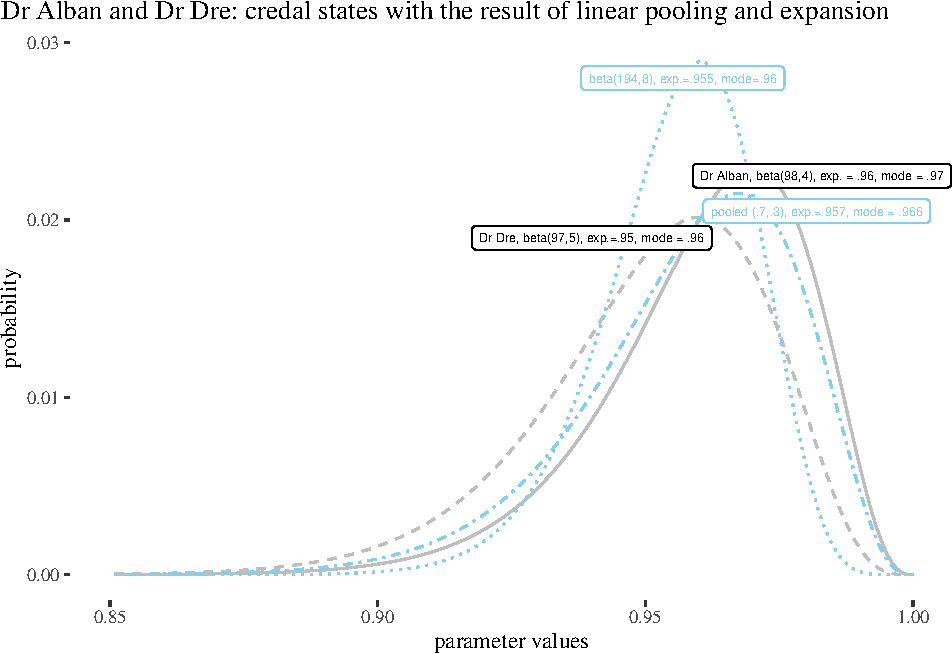
\includegraphics[width=1\linewidth]{impreciseEpistemicFINAL_files/figure-latex/fig:Dre-1} \end{center}
\caption{Pooling and expansion on the assumption the agent's evidence is disjoint.}
\label{fig:dre}
\end{figure}

First, what beta distribution would correspond to the pooled
distribution? Calculating concentration (\(\kappa\)) from the mean
(\(\mu\)) and the mode (\(\omega\)) by taking
\(\kappa = \nicefrac{1-2\omega}{\mu-\omega}\)\footnote{This is because $\mu \kappa = a = \omega(k - 2) +1$}
with values taken from the pooled distribution gives us
\(\kappa= .84.72\). Further, \(a = \mu \kappa\), so \(a = 80.91\) and
\(b - 3.81\). So, with linear pooling, we behave, approximately, as if
we observed 79 successes and three failures. Pooling makes us dispose of
information that we do have and lowers our confidence inappropriately.
We avoid this difficulty by first figuring out what evidence would have
led Dr Dre to have the credal stance she has and updating on it. If her
evidence did not overlap with ours, we can use the whole power of all
the observations to arrive at a more sensible distribution.

There is a clear sense in which a synergy effect can be observed here.
On one hand, neither our mode nor our mean shifts dramatically, the
change being most likely of no practical difference. Nevertheless, the
distribution narrows down and so does the HDI, corresponding to a
confidence boost. These comparative results are also mirrored by
information-theoretic weight calculations (although we're not talking
about likelihoods, so we are not dealing with weights of evidence here).

\begin{table}
\begin{tabular}{lrrrr}
\toprule
  & HDI low & HDI high & HDI width & weight\\
\midrule
Dr Alban & 0.933 & 0.989 & 0.056 & 0.378\\
Dr Dre & 0.916 & 0.98 & 0.064 & 0.360\\
pooled & 0.927 & 0.986 & 0.059 & 0.369\\
expanded & 0.933 & 0.977 & 0.044 & 0.414\\
\bottomrule
\end{tabular}
\caption{Confidence and information measures for two aggregation methods in the Alban-Dre scenario.}
\label{tab:synergy}
\end{table}

At this point, the question is, whether expansions always leads to
synergy. The intuition is that it should not. After all, if the opinions
are too different, you should become more confused not more confident
upon obtaining them, right? So imagine this time you run into Dr Seuss
instead of Dr Dre, and she tells you she observed 35 successes and 65
failures. The recommendations of linear pooling and expansion are in
Figure \ref{fig:seuss}.

\begin{figure}[H]

\begin{center}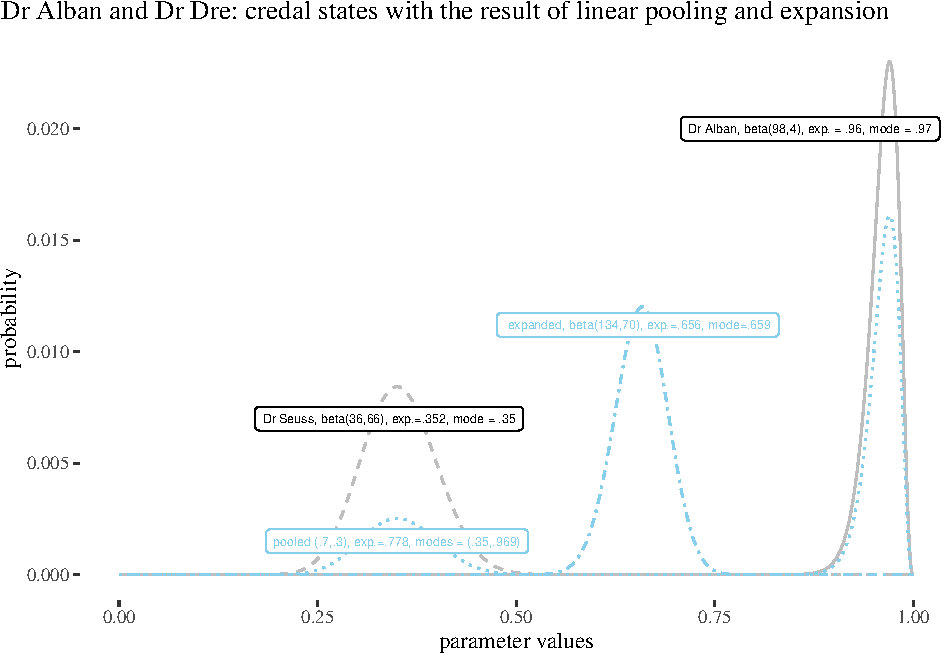
\includegraphics[width=1\linewidth]{impreciseEpistemicFINAL_files/figure-latex/fig:seuss-1} \end{center}

\caption{Results of linear pooling with weights $(.7, .5)$ and expansion in case of divergent experts' testimony.}
\label{fig:seuss}
\end{figure}

The pooled distribution is now bimodal with a disjoint HDI of joint
width .1754 and weight 0.248. In contrast, the HDI width of the expanded
distribution is .105, and its weight is .287, so the expanded
distribution is not only more principled but also preserves more
confidence and information. Note however that your original HDI width
was 0.056, and your original weight was .378, so in this case after
learning there is a sense in which there is no synergy, as you end up
less confident with a less informative distribution. This is as
expected.

For each particular overlap size you can calculate the expected \(a\)
and \(b\) of the beta distribution that you should add to your
distribution's parameters upon updating on the evidence you think the
other expert has. If you don't know the extent of evidential overlap
between the experts but at least have a probability distribution for
various levels of overlap, you can still calculate your expected new
beta distribution. Here's an example in which the probability
distribution of evidential overlaps is in a principled way non-uniform.
I'll use it to illustrate the idea that expansion leads to more accurate
credal states than linear pooling no matter what the real chance is.

Here is how the example goes. Consider a given chance hypothesis \(c\).
Suppose two experts draw observations from the same group of size 100 in
which the distribution of successes is binomial with probability \(c\).
Each expert observes a sample of size 20 and records her number of
successes. They start with uniform priors and revise to more informative
beta distributions accordingly to what they have observed. You are
expert one. On one hand, you average your and the other expert's opinion
with weights \((.5,.5)\). On another, you figure out that evidential
overlap goes from \(0\) to \(20\) with the hypergeometric distribution
\(\frac{{20 \choose k}{80 \choose (20-k)}}{{100 \choose 20}}\). For each
potential overlap, you calculate the \(a\) and \(b\) that you should add
to your beta distribution parameters, and then you use the
hypergeometric distribution to calculate the expected values. You expand
your distribution by adding those. Then you measure the inaccuracy of
both newly obtained distributions with respect to the real probability
hypothesis \(c\). Now imagine for each of 101 of evenly spaced real
chance hypotheses you do this 100 times, recording inaccuracies. The
result of the simulation is in Figure \ref{fig:inaccuraciesSimulation}.
The simulated expected inaccuracy of pooling is higher than that of
expanding, no matter what the real chance hypothesis is.

\begin{figure}[H]

\begin{center}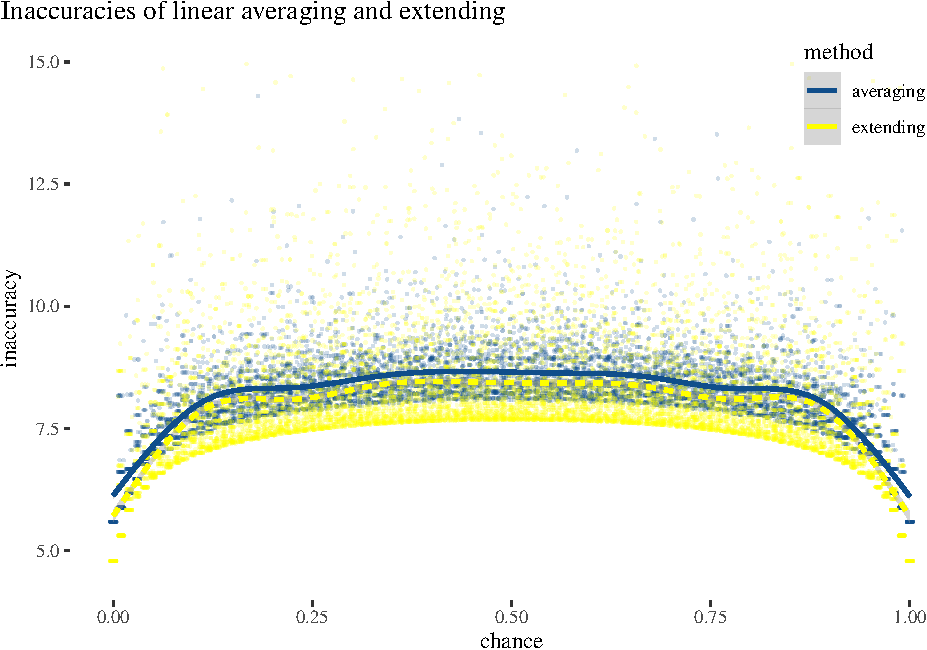
\includegraphics[width=1\linewidth]{impreciseEpistemicFINAL_files/figure-latex/fig:inaccuraciesSimulation-1} \end{center}
\caption{Simulated inaccuraces of two methods of updating on expert's opinion. Pooling performs worse than expansion, across all real probability hypotheses.}
\label{fig:inaccuraciesSimulation}
\end{figure}

This, of course, is just a toy example. Its main point is that even in
fairly straightforward settings accuracy considerations might suggest an
aggregation strategy that differs from linear pooling. Real-life
situations, of course, are much messier, but at least the suggestion of
figuring out how much of the initial disagreement is due to evidential
differences, what the extent of evidential overlap is, and how much is
due to a difference in background modeling assumptions (and what reasons
the agent has to use them), seems \emph{prima facie} sensible.

\hypertarget{wrapping-up-and-loose-ends}{%
\section{Wrapping up and loose ends}\label{wrapping-up-and-loose-ends}}

We've covered quite a bit of ground: I started with a list of reasons
why some people favor IP over PP. Then I explained various reasons why
some people still find IP unsatisfactory. This was the negative set-up
for the positive proposal that followed.

The positive proposal, roughly, is this: instead of using IP and running
into its own difficulties, why not use methods that Bayesian statistics
is already familiar with? Let's think about the uncertainty about a
proposition in terms of parameter uncertainty, where this parameter is
the right probability that one should assign to that proposition (be it
chance, the sole rational probability given the evidence or what have
you, let's leave the philosophical discussion open). Once we do this,
there are tools that we can use to explain how the framework can handle
both the motivations for departing from PP, and the difficulties that IP
runs into.

Of course, given the number of issues that we've gone over, I could have
gone into more details of this or that problem, or discussed another
problem that the reader is familiar with but I did not bring up. Sure.
However, my goal in this paper was to put the proposal on the table and
explain how it fits into the larger picture of the debate between PP and
IP. Below, I will allow myself only to list and briefly comment on
issues that did not receive in this paper the treatment the reader might
think they deserve.

One might worry that this approach still involves some over-specificity
in RA's credal state representation. There are quite a few ways this
concern might arise. One variant of this objection comes from (James M.
Joyce, 2010), who points out that even uniform distribution over the
full range of chance hypotheses seems overly informative, e.g.~it
commits you to thinking that in a hundred independent tosses of the
coin, the chances of heads coming up fewer than 17 times is exactly
17/101, just a bit more probable than rolling an ace with fair die. ``Do
you really think that your evidence justifies such a specific
probability assignment?'', he asks.

The objection, however, has a limited strength here. Once we do not
accept the idea that an agent's credal states are adequately represented
by one-number summaries, a more appropriate way to describe the RA's
credal state is to display the prior predictive distribution for the
outcomes of 100 tosses, which is uniform instead of any summaries. Sure,
around 17\% of the results will be around 17\%, but RAs extreme
uncertainty is still captured: the highest posterior density fails to
select any particularly interesting sub-region of the distribution, and
if you ask RA to predict the outcome or make any comparison, they will
be right to say that they have no idea.

Moreover, since uniform priors are usually used in the initial step of a
learning process (if they are to be used at all). Using flat prior to
guide one's action and inspire bet \$ 17 to \$ 100 on the result being
below 17 if there is no information is rarely a recommended course of
action anyway. The goal of priors is not to underlie decision making,
and so the threat of some specific numbers falling out of the priors
prior to data analysis is not of much practical relevance.

One might complain further about uniform priors, complaining that
monotone transformations of variables with uniform distributions might
not have uniform distributions. First, note that nothing in the
representation methods defended in this paper itself depends on the fact
that following the philosophical literature I used uniform priors in
some examples. Second, while philosophers tend to worry about the
recommended mental states of idealized agents in the state of complete
lack of information, this is less of a worry for people more concerned
with what actual agents reasoning about the world should think. It is
well-known that uniform distributions are susceptible to over-fitting,
and even in seemingly non-Bayesian machine-learning methods
regularization is quite common (say, in ridge or lasso regression
methods).\footnote{It is also susceptible to Bayesian interpretation on which the priors are explicitly used and not uniform. For instance, ridge regression effectively behaves like Bayesian regression with a Gaussian prior centered on 0 with a standard deviation being a function of the tuning parameter used in the ridge regression itself.}
After all, one of the important advantages of the Bayesian statistics is
that now one can perform her analysis without using classical methods
with behave as if the prior was uniform. Third, while obviously, say, if
the real probability \(\theta\) has uniform distribution, \(\theta^2\)
will not, it is not clear why this is problematic. If you think that the
notion of probability helps you cut nature at its joints and make
prediction, perhaps you should focus on using it in building your models
or predictions, instead of trying to use grue-like transformations.

Uniform priors aside, one might complain more generally about
overspecificity. After all, the distributions have their own parameters
that specify them, and for any distribution one can ask, why this
distribution rather than one in which the parameter is slightly
different hasn't been used? For instance, why represent a given state as
\(\mathsf{norm}(.5,.05)\) rather than \(\mathsf{norm}(.5,.0501)\)? Fair
enough. Note however, that any probabilistic proposal on the market, IP
including, can be accused of a variant of this problem. When we apply a
mathematical toolkit we're in the business of idealization, and we're
bound to make some such somewhat arbitrary moves in the process. The
question is then not whether the use of a mathematical tool involves an
idealization, but whether the tool helps us solve our problems better
than or at least as well as other tools, if used with full awareness of
such an idealization being made.

Perhaps, you might dislike the idea of going higher-order for
theoretical reasons. One might be that you don't like the complexity.
This seems to be the line taken by Bradley, who refuses to go
higher-order for the following reason:

\begin{quote}
Why is sets of probabilities the right level to stop the regress at? Why not sets of sets? Why not second-order probabilities? Why not single probability functions? This is something of a pragmatic choice. The further we allow this regress to continue, the harder it is to deal with these belief representing objects. So let's not go further than we need. 131-132\end{quote}

I have argued extensively, that given the difficulties of both PP and IP
and how the current approach handles it, we are not going further than
we need in using higher-order probabilities. We're going where we should
be. And the supposed pragmatic concerns that one might have are unclear:
parameter uncertainty, approximations and other computational methods I
have used in fact quite embedded in Bayesian statistical practice and
decent computational tools for the framework I propose are
available.\footnote{Also, you can insist that instead of going higher order we could just take our sample space to be the cartesian product of the original sample space and parameter space, or use parameters having certain values as potential states of a bayesian network. If you prefer not to call such approaches first-order, I don't mind, as long as you effectively end up assigning probabilities to certain probabilities, the representation means I discussed in this paper should be in principle available to you.}

Another concern that you might have is that it is not clear what the
semantics of such an approach should look like. While a more elaborate
account is beyond the scope of this paper, the general gist of the
approach can be modeled by a slight modification of a framework of
probabilistic frames (Dorst, 2022b, 2022a). Start with a set of possible
worlds \(W\). Suppose you consider a class of probability distributions
\(D\), a finite list of atomic sentences \(q_1, \dots, q_2\)
corresponding to subsets of \(W\), and a selection of true probability
hypotheses \(C\) (think of the latter as omniscient distributions,
\(C\subseteq D\), but in principle this restriction can be dropped if
need be). Each possible world \(w\in W\) and a proposition
\(p\subseteq W\) come with their true probability distribution,
\(C_{w,p}\in D\) corresponding to the true probability of \(p\) in
\(w\), and the distribution that the expert assigns to \(p\) in \(w\),
\(P_{w,p}\in D\). Then, various propositions involving distributions can
be seen as sets of possible worlds, for instance, the proposition that
the expert assigns \(d\) to \(p\) is the set of worlds \(w\) such that
\(P_{w,p}=d\).\footnote{There is at least one important difference between this approach and that developed by Dorst. His  framework is untyped, which allows for an enlightening discussion of the principle of reflection and alternatives to it. In this paper I prefer to keep this complexity apart and use an explicitly typed set-up.}

Finally, you might be worried that I have not discussed complex and
dependent propositions, for instance completely ignoring the discussion
of dilation, which is a phenomenon highly relevant to the philosophical
status of imprecise probabilities. Indeed, I preferred adding additional
layer of complexity to this already long paper, postponing the
discussion of such issues.

\hypertarget{appendix-the-strict-propriety-of-mathcali_dkl2}{%
\section*{\texorpdfstring{Appendix: the strict propriety of
\(\mathcal{I}_{\dkl}^2\)}{Appendix: the strict propriety of \textbackslash mathcal\{I\}\_\{\textbackslash dkl\}\^{}2}}\label{appendix-the-strict-propriety-of-mathcali_dkl2}}
\addcontentsline{toc}{section}{Appendix: the strict propriety of
\(\mathcal{I}_{\dkl}^2\)}

Let us start with a definition.

\begin{definition}[concavity]
%A function $f$ is convex over an interval $(a,b)$ just in case for all  $x_1, x_2\in (a,b)$ and $0 \leq \lambda \leq 1$ we have:
%\begin{align*}
%f(\lambda x_1 + (1-\lambda)x_2) \leq \lambda f(x_1) + (1-\lambda)f(x_2)
%\end{align*}
A function $f$  is concave just in case
\begin{align*}
f(\lambda x_1 + (1-\lambda)x_2) \geq \lambda f(x_1) + (1-\lambda)f(x_2)
\end{align*}
\noindent it is strictly concave just in case the equality holds only if either $\lambda = 0$ or $\lambda = 1$.
\end{definition}

For us it is important that if a function is twice differentiable on an
interval, then it is (strictly) concave just in case its second
derivative is non-positive (negative). In particular, as
\((\log_2(x))'' = -\frac{1}{x^2 ln(2)}\), \(\log_2\) is stritly concave
over its
domain.\footnote{I line with the rest of the paper, we'll work with $\log$ base 2. We could equally well use any other basis.}

\begin{lemma}[Jensen's inequality]
If $f$ is concave, and $g$ is any function of a random variable, $\E(f(g(x))) \leq f(\E(g(x)))$. If $f$ is strictly concave, the equality holds only if $g(x) = \E g(x)$, that is, if $g(x)$ is constant everywhere.
\end{lemma}

\begin{proof}
For the base case consider a two-point mass probability function. Then,
\begin{align*}
p_1f(g(x_1))+ p_2f(g(x_2)) &\leq f(p_1g(x_1) + p_2g(x_2))
\end{align*}
\noindent follows directly from the definition of concativity, if we take $\lambda = p_1$, $(1-\lambda)=p_2$, and substitute $g(x_1)$ and $g(x+2)$ for $x_1$ and $x_2$.



Now, suppose that  $ p_1f(g(x_1))+ p_2f(g(x_2)) = f(p_1g(x_1) + p_2g(x_2))$ and that   $f$ is strictly concave. That means either $(p_1 = 1\wedge p_2 = 0)$, or $(p_1 = 0 \wedge p_2 =1)$. Then either $x$ always takes value $x_1$, in the former case, or always takes value $x_2$, in the latter case. $\E g (x) =  p_1 g(x_1) + p_2 g(x_2)$, which equals  $g(x_1)$ in the former case and $g(x_2)$ in the latter.


Now suppose Jensen's inequality and the consequence of strict contativity) holds for $k-1$ mass points. Write $p_i' = \frac{p_i}{1-p_k}$ for $i = 1, 2, \dots, k-1$. We now reason:
\begin{align*}
\sum_{i=1}^k p_i f(g(x_i)) & =
 p_kf(g(x_k)) + (1-p_k)\sum_{i =1}^{k-1}p_i'f(g(x_i)) &\\
 & \leq p_k f(g(x_k)) + (1-p_k)f\left( \sum_{i = 1}^{k=i}p_i' g(x_i) \right) & \mbox{\footnotesize by the induction hypothesis}\\ &\leq f\left( p_k(g(x_k)) + (1-p_k)\sum_{i = 1}^{k-1} p_i' g(x_i)\right) & \mbox{\footnotesize by the base case} \\
 & = f \left( \sum_{i}^k p_i g(x_i)\right)
 \end{align*}

Notice also that at the induction hypothesis application stage we know that the equality holds only if $p_k =1 \vee p+k = 0$. In the former case $g(x)$ always takes value $x_k = \E g(x)$. In the latter case, $p_k$ can be safely ignored and $\sum_{i=1}^{k}p_ig(x_i) = \sum_{i=1}^{k-1}p'g(x_i)$ and by the induction hypothesis we already know that $\E g(x) = g(x)$.


\end{proof}

In particular, the claim holds if we take \(g(x)\) to be
\(\frac{q(x)}{p(x)}\) (were both \(p\) and \(q\) are probability mass
functions), and \(f\) to be \(\log_2\). Then, given that \(A\) is the
support set of \(p\), we have: \begin{align*}
\sum_{x\in A}p(x) \log_2 \frac{q(x)}{p(x)} & \leq \log_2 \sum_{x\in A}p(x)\frac{q(x)}{p(x)}
\end{align*}

\noindent Moreover, the equality holds only if \(\frac{q(x)}{p(x)}\) is
constant, that is, only if \(p\) and \(q\) are the same pmfs. Let's use
this in the proof of the following lemma.

\begin{lemma}[Information inequality] For two probability mass functions $p, q$, $\dkl(p,q)\geq 0$ with equality iff $p=q$.
\end{lemma}

\begin{proof}
Let $A$ be the support set of $p$, and let $q$ be a probability mass function whose support is $B$.
\begin{align*}
- \dkl(p,q) & = - \sum_{x\in A}p(x) \log_2 \frac{p(x)}{q(x)}& \mbox{\footnotesize (by definition)} \\
&  =  \sum_{x\in A}p(x)  - \left(\log_2 p(x) - \log_2 q(x)\right)& \\
&  =  \sum_{x\in A}p(x)   \left(\log_2 q(x) - \log_2 p(x)\right)& \\
& =  \sum_{x\in A} p(x) \log_2 \frac{q(x)}{p(x)}& \\
& \leq \log_2 \sum_{x\in A} p(x)\frac{q(x)}{p(x)} & \mbox{\footnotesize by Jensen's inequality}\\
& \mbox{(and the equality holds only if $p = q$)}\\
& = \log_2 \sum_{x\in A} q(x)  & \\
& \leq \log_2 \sum_{x\in B} q(x) & \\
& = log (1)  = 0 &\\
\end{align*}
\end{proof}

Observe now that \(\dkl\) can be decomposed in terms of cross-entropy
and entropy.

\begin{lemma}[decomposition] $\dkl = H(p,q) - H(p)$. \end{lemma}

\begin{proof}
\begin{align*}
\dkl (p, q) & = \sum_{p_{i}} \left( \log_2 p_i - \log_2 q_i \right) \\
& =   - \sum_{p_{i}}\left( \log_2 q_{i} - \log_2 p_{i} \right) \\
& = - \sum_{p_{i}} \log_{2} q_{i} - \sum_{p_{i}} - \log_{2} p_{i}   \\
& -  \underbrace{- \sum_{p_{i}} \log_2 q_{i}}_{H(p,q)}    - \underbrace{- \sum_{p_i}  \log_2 p_{i}}_{H(p)}
\end{align*}
\end{proof}

With information inequality this easily entails Gibbs' inequality:

\begin{lemma}[Gibbs' inequality] $H(p,q) \geq H(p)$ with identity only if $p = q$.
\end{lemma}

Now we are done with our theoretical set-up. Here is how it entails the
propriety of \(\mathcal{I}_{\dkl}^2\). First, let's systematize the
notation. Consider a discretization of the parameter space \([0,1]\)
into \(n\) equally spaced values \(\theta_1, \dots, \theta_n\). For each
\(i\) the ``true'\,' second-order distribution if the true parameter
indeed is \(\theta_i\)---we'll call it the indicator of \(\theta_i\)---
is defined by \begin{align*}
Ind^k(\theta_i) & = \begin{cases} 1 & \mbox{if } \theta_i = \theta_k\\
                        0 & \mbox{otherwise}  \end{cases}
\end{align*} \noindent I will write \(Ind^k_i\) instead of
\(Ind^k(\theta_i)\).

Now consider a probability distribution \(p\) over this parameter space,
assigning probabilities \(p_1, \dots, p_n\) to
\(\theta_1, \dots, \theta_n\) respectively. It is to be evaluated in
terms of inaccuracy from the perspective of a given
\texttt{true\textquotesingle{}\textquotesingle{}\ value\ \$\textbackslash{}theta\_k\$.\ The\ inacurracy\ of\ \$p\$\ if\ \$\textbackslash{}theta\_k\$\ is\ the}true'\,'
value, is the divergence between \(IndI^k\) and \(p\).

\begin{align*}
\mathcal{I}_{\dkl}^2(p, \theta_k) & = \dkl(Ind^k,p) \\
& = \sum_{i=1}^n Ind^k_i \left( \log_2 Ind^k_i - \log_2 p_i \right)
\end{align*} Note now that for \(j \neq k\) we have \$Ind\^{}k\_j = 0 \$
and so \(Ind^k_j \left( \log_2 Ind^k_j - \log_2 p_j \right)=0\).
Therefore we continue: \begin{align*}
& = Ind^k_k \left( \log_2 Ind^k_k - \log_2 p_k \right)
\end{align*} Further, \(Ind^k_k= 1\) and therefore
\(\log_2 Ind^k_k =0\), so we simplify: \begin{align*}
& =  - \log_2 p_k
\end{align*}

\noindent Now, let's think about expected values. First, what the
inaccuracy of \(p\) as expected by \(p\), \(\EI(p,p)\)\$?

\begin{align*}
\EI(p,p) & = \sum_{i =1}^n p_i \mathcal{I}_{\dkl}^2(p, \theta_k) \\
& = \sum_{i =1}^n  p_i - \log_2 p_k \\
& = - \sum_{i =1}^n  p_i  \log_2 p_k = H(p)
\end{align*}

\noindent Analogously, the inaccuracy of \(q\) as expected from the
perspective of \(p\) is:

\begin{align*}
\EI(p, q) & =   \sum_{i =1}^n p_i \left( - \log_2 q_i\right)\\
& = -  \sum_{i =1}^n p_i  \log_2 q_i) = H(p,q)
\end{align*}

But that means, by Gibb's inequality, that \(\EI(p,q) \geq EI(p,p)\)
unless \(p=q\), which completes the proof.

\hypertarget{references}{%
\section*{References}\label{references}}
\addcontentsline{toc}{section}{References}

\hypertarget{refs}{}
\begin{CSLReferences}{1}{0}
\leavevmode\vadjust pre{\hypertarget{ref-bradley2012uncertaintyPhD}{}}%
Bradley, S. (2012). \emph{Scientific uncertainty and DecisionMaking}
(PhD thesis). London School of Economics; Political Science.

\leavevmode\vadjust pre{\hypertarget{ref-bradley2019imprecise}{}}%
Bradley, S. (2019). {Imprecise Probabilities}. In E. N. Zalta (Ed.),
\emph{The {Stanford} encyclopedia of philosophy} ({S}pring 2019).
\url{https://plato.stanford.edu/archives/spr2019/entries/imprecise-probabilities/};
Metaphysics Research Lab, Stanford University.

\leavevmode\vadjust pre{\hypertarget{ref-CampbellMoore2020accuracy}{}}%
Campbell-Moore, C. (2020). \emph{Accuracy and imprecise probabilities}.

\leavevmode\vadjust pre{\hypertarget{ref-Carr2020impreciseEvidence}{}}%
Carr, J. R. (2020). Imprecise evidence without imprecise credences.
\emph{Philosophical Studies}, \emph{177}(9), 2735--2758.
\url{https://doi.org/10.1007/s11098-019-01336-7}

\leavevmode\vadjust pre{\hypertarget{ref-Christensen2009disagreement}{}}%
Christensen, D. (2009). Disagreement as evidence: The epistemology of
controversy. \emph{Philosophy Compass}, \emph{4}(5), 756--767.
\url{https://doi.org/10.1111/j.1747-9991.2009.00237.x}

\leavevmode\vadjust pre{\hypertarget{ref-Dietrich2016pooling}{}}%
Dietrich, F., \& List, C. (2016). Probabilistic opinion pooling. In A.
Hajek \& C. Hitchcock (Eds.), \emph{Oxford handbook of philosophy and
probability}. Oxford: Oxford University Press.

\leavevmode\vadjust pre{\hypertarget{ref-Dorst2022evidence}{}}%
Dorst, K. (2022a). Higher-order evidence. In M. Lasonen-Aarnio \& C.
Littlejohn (Eds.), \emph{The routledge handbook for the philosophy of
evidence}. Routledge.

\leavevmode\vadjust pre{\hypertarget{ref-Dorst2022higher-order}{}}%
Dorst, K. (2022b). Higher-order uncertainty. In M. Skipper \& A. S.
Petersen (Eds.), \emph{Higher-order evidence: New essays}.

\leavevmode\vadjust pre{\hypertarget{ref-Dorst2021deference}{}}%
Dorst, K., Levinstein, B. A., Salow, B., Husic, B. E., \& Fitelson, B.
(2021). Deference done better. \emph{Wiley: Philosophical Perspectives},
\emph{35}(1), 99--150. \url{https://doi.org/10.1111/phpe.12156}

\leavevmode\vadjust pre{\hypertarget{ref-Elga2007reflection}{}}%
Elga, A. (2007). Reflection and disagreement. \emph{Noûs}, \emph{41}(3),
478--502. \url{https://doi.org/10.1111/j.1468-0068.2007.00656.x}

\leavevmode\vadjust pre{\hypertarget{ref-elga2010subjective}{}}%
Elga, A. (2010). \emph{Subjective probabilities should be sharp}.

\leavevmode\vadjust pre{\hypertarget{ref-Lee2017impreciseEpistemology}{}}%
Elkin, L. (2017). \emph{Imprecise probability in epistemology} (PhD
thesis). Ludwig-Maximilians-Universit{ä}t;
Ludwig-Maximilians-Universität München.

\leavevmode\vadjust pre{\hypertarget{ref-Elkin2018resolving}{}}%
Elkin, L., \& Wheeler, G. (2018). Resolving peer disagreements through
imprecise probabilities. \emph{Noûs}, \emph{52}(2), 260--278.
\url{https://doi.org/10.1111/nous.12143}

\leavevmode\vadjust pre{\hypertarget{ref-VanFraassen2006vague}{}}%
Fraassen, B. C. V. (2006). Vague expectation value loss.
\emph{Philosophical Studies}, \emph{127}(3), 483--491.
\url{https://doi.org/10.1007/s11098-004-7821-2}

\leavevmode\vadjust pre{\hypertarget{ref-vanFraassen1984beliefandWill}{}}%
Fraassen, B. C. van. (1984). Belief and the will. \emph{Journal of
Philosophy}, \emph{81}(5), 235--256.
\url{https://doi.org/10.2307/2026388}

\leavevmode\vadjust pre{\hypertarget{ref-gaifman1988higherOrder}{}}%
Gaifmam, H. (1988). A theory of higher order probabilities. In B. Skyrms
\& W. L. Harper (Eds.), \emph{Causation, chance, and credence} (Vol. 1,
pp. 191--219). Kluwer.

\leavevmode\vadjust pre{\hypertarget{ref-Gallow2018masters}{}}%
Gallow, J. (2018). No one can serve two epistemic masters.
\emph{Philosophical Studies}, \emph{175}(10), 2389--2398.
\url{https://doi.org/10.1007/s11098-017-0964-8}

\leavevmode\vadjust pre{\hypertarget{ref-Gardenfors1982unreliable}{}}%
Gärdenfors, P., \& Sahlin, N.-E. (1982). Unreliable probabilities, risk
taking, and decision making. \emph{Synthese}, \emph{53}(3), 361--386.
\url{https://doi.org/10.1007/bf00486156}

\leavevmode\vadjust pre{\hypertarget{ref-jaynes2003probability}{}}%
Jaynes, E. T. (2003). \emph{Probability theory: The logic of science}.
Cambridge university press.

\leavevmode\vadjust pre{\hypertarget{ref-joyce2005probabilities}{}}%
Joyce, James M. (2005). How probabilities reflect evidence.
\emph{Philosophical Perspectives}, \emph{19}(1), 153--178.

\leavevmode\vadjust pre{\hypertarget{ref-Joyce2010defense}{}}%
Joyce, James M. (2010). A defense of imprecise credences in inference
and decision Making1. \emph{Philosophical Perspectives}, \emph{24}(1),
281--323. \url{https://doi.org/10.1111/j.1520-8583.2010.00194.x}

\leavevmode\vadjust pre{\hypertarget{ref-Kaplan1968decision}{}}%
Kaplan, J. (1968). Decision theory and the fact-finding process.
\emph{Stanford Law Review}, \emph{20}(6), 1065--1092.

\leavevmode\vadjust pre{\hypertarget{ref-Kaplan1996decision}{}}%
Kaplan, M. (1996). \emph{Decision theory as philosophy}. Cambridge
University Press.

\leavevmode\vadjust pre{\hypertarget{ref-keynes1921treatise}{}}%
Keynes, J. M. (1921). \emph{A treatise on probability, 1921}. London:
Macmillan.

\leavevmode\vadjust pre{\hypertarget{ref-konek2013foundations}{}}%
Konek, J. (2013). \emph{New foundations for imprecise bayesianism} (PhD
thesis). University of Michigan.

\leavevmode\vadjust pre{\hypertarget{ref-Levi1974ideterminate}{}}%
Levi, I. (1974). On indeterminate probabilities. \emph{The Journal of
Philosophy}, \emph{71}(13), 391. \url{https://doi.org/10.2307/2025161}

\leavevmode\vadjust pre{\hypertarget{ref-Levi1980enterprise}{}}%
Levi, I. (1980). \emph{The enterprise of knowledge: An essay on
knowledge, credal probability, and chance}. MIT Press.

\leavevmode\vadjust pre{\hypertarget{ref-Lewis1980subjectivist}{}}%
Lewis, D. K. (1980). A subjectivist?s guide to objective chance. In R.
C. Jeffrey (Ed.), \emph{Studies in inductive logic and probability,
volume II} (pp. 263--293). Berkeley: University of California Press.

\leavevmode\vadjust pre{\hypertarget{ref-List2011groupAgency}{}}%
List, C., \& Pettit, P. (2011). \emph{Group agency: The possibility,
design, and status of corporate agents}. Oxford University Press.

\leavevmode\vadjust pre{\hypertarget{ref-Mayo-Wilson2016scoring}{}}%
Mayo-Wilson, C., \& Wheeler, G. (2016). Scoring imprecise credences: A
mildly immodest proposal. \emph{Philosophy and Phenomenological
Research}, \emph{92}(1), 55--78.
\url{https://doi.org/10.1111/phpr.12256}

\leavevmode\vadjust pre{\hypertarget{ref-Rinard2013against}{}}%
Rinard, S. (2013). Against radical credal imprecision. \emph{Thought: A
Journal of Philosophy}, \emph{2}(1), 157--165.
\url{https://doi.org/10.1002/tht3.84}

\leavevmode\vadjust pre{\hypertarget{ref-Schoenfield2017accuracy}{}}%
Schoenfield, M. (2017). The accuracy and rationality of imprecise
credences. \emph{Noûs}, \emph{51}(4), 667--685.
\url{https://doi.org/10.1111/nous.12105}

\leavevmode\vadjust pre{\hypertarget{ref-seidenfeld2012forecasting}{}}%
Seidenfeld, T., Schervish, M., \& Kadane, J. (2012). Forecasting with
imprecise probabilities. \emph{International Journal of Approximate
Reasoning}, \emph{53}, 1248--1261.
\url{https://doi.org/10.1016/j.ijar.2012.06.018}

\leavevmode\vadjust pre{\hypertarget{ref-Stewart2018pooling}{}}%
Stewart, R. T., \& Quintana, I. O. (2018). Learning and pooling, pooling
and learning. \emph{Erkenntnis}, \emph{83}(3), 1--21.
\url{https://doi.org/10.1007/s10670-017-9894-2}

\leavevmode\vadjust pre{\hypertarget{ref-Sturgeon2008grain}{}}%
Sturgeon, S. (2008). Reason and the grain of belief. \emph{No{û}s},
\emph{42}(1), 139--165. Retrieved from
\url{http://www.jstor.org/stable/25177157}

\leavevmode\vadjust pre{\hypertarget{ref-walley1991statistical}{}}%
Walley, P. (1991). \emph{Statistical reasoning with imprecise
probabilities}. Chapman; Hall London.

\leavevmode\vadjust pre{\hypertarget{ref-williamson2010defence}{}}%
Williamson, J. (2010). \emph{In defence of objective bayesianism}.
Oxford University Press Oxford.

\end{CSLReferences}

\end{document}
